\documentclass[12pt,a4paper]{article}
\usepackage[utf8]{inputenc}
\usepackage{amsmath}
\usepackage{amsfonts}
\usepackage{amssymb}
\usepackage{graphicx}
\usepackage{float}
\usepackage{booktabs}
\usepackage{geometry}
\usepackage{natbib}
\usepackage{url}
\usepackage{tikz}
\usepackage{pgfplots}
\pgfplotsset{compat=1.18}
\usepackage{subcaption}
\usepackage{xcolor}
\usepackage{setspace}
\usepackage{dirtytalk}
\usepackage{graphicx}
\graphicspath{ {./images/} }
\usepackage[rightcaption]{sidecap}
\usepackage[colorlinks=true, linkcolor=blue, citecolor=blue, urlcolor=blue]{hyperref}


\geometry{margin=1in}
\onehalfspacing

\title{\Large \textbf{Finance and the Unexpected}}

\author{
Saranya Anantapantula\\
\small University of Pennsylvania\\
Dr. Jessica Wachter\\
\small University of Pennsylvania - Finance Department
}

\date{\today}

\begin{document}

\maketitle

\begin{abstract}
Extreme events in financial markets challenge traditional models built on volatility and normal distributions. Tail risks, model failures, and behavioral biases continue to drive persistent mispricing and systemic vulnerability. Prior research often relies on mean-variance frameworks, overlooking higher moments like skewness and kurtosis, as well as the limits of diversification under moral hazard. We use simulated jump-diffusion models, Monte Carlo experiments, and empirical return data to expose the underestimation of rare, severe shocks in asset pricing and in investor expectations. Option markets, credit derivatives, and debt instruments reveal embedded short-put-like structures that mask hidden risks. Behavioral insights from memory and context effects explain why investors lean on recent experience, misjudge tail probabilities, and fail to revise models even after crisis events. While short-term returns are marked by negative skewness and excess kurtosis, the long-run performance of public equities, enabled by regulation and broad risk-sharing, remains a surprising and underappreciated success.
\end{abstract}
% https://www.econometricsociety.org/publications/es-data-editor-website/package

\section{Introduction and Theoretical Framework}

Financial markets exhibit pervasive uncertainty that extends beyond simple volatility measurements. This paper provides a framework for understanding these uncertainties by distinguishing among different types of risk and their implications for market participants. A central question guides our analysis: how can we understand and manage the unexpected in financial markets when the very tools we use to measure risk may be inadequate?

Drawing on both simulated and observed market data, we show how individual stock returns differ sharply from those of diversified portfolios, examine how moral hazard limits diversification in practice and how regulation can mitigate it, and consider why even sophisticated market participants underestimate tail risks.

\subsection{Defining the Unexpected}
Life presents us with countless outcomes we cannot predict with certainty. In financial markets, this uncertainty presents across various dimensions: the outcome of a specific FDA trial, the integrity of corporate management, daily stock market returns, the stability of financial institutions, and especially the beliefs of other market participants.

Mathematically, we represent the range of possible outcomes as a random variable. For any uncertain outcome $X$, we can form an expectation $E[X]$. Something becomes \say{unexpected} to the degree that a realized outcome $x$ deviates from the overall expectation (i.e., when $|x - E[X]|$ is large). Even if a specific outcome is slightly unexpected, it still carries risk, and most won't accept that risk for free.

\subsection{Risk Aversion and the Demand for Compensation}

The foundation of modern finance rests on the assumption that individuals are risk-averse, meaning most require extra compensation if they are taking risk. This stems from the idea of diminishing marginal utility: people derive less additional satisfaction from each incremental unit of consumption or wealth (\autoref{fig:fig1}). Concretely, let $u(w)$ represent an investor’s utility from wealth $w$. We assume $u'(w) > 0$ (utility increases with wealth) but $u''(w) < 0$ (marginal utility decreases), so utility is increasing and concave. 

\begin{figure}[h]
    \centering
    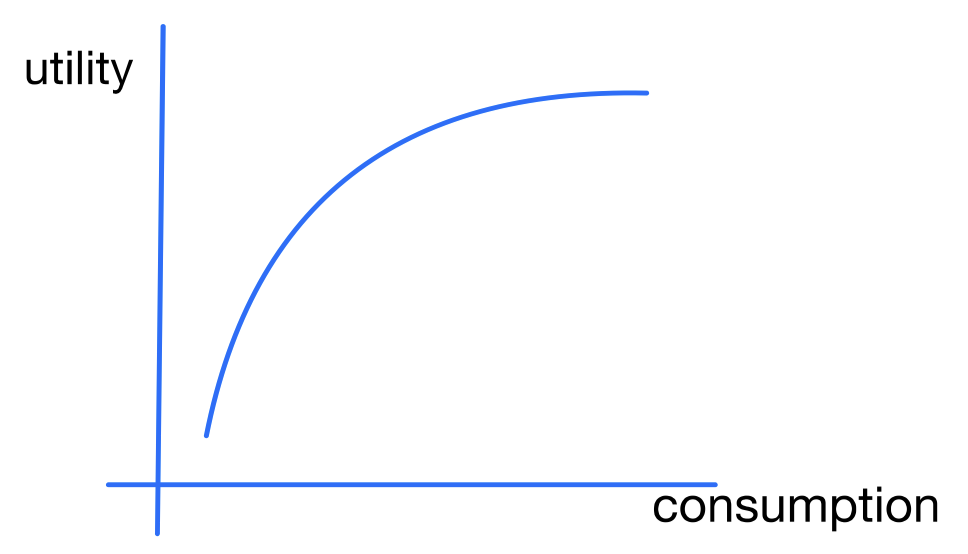
\includegraphics[width=0.50\textwidth]{fig1.png}
    \caption{Concave utility function showing diminishing marginal utility}
    \label{fig:fig1}
\end{figure}

Because of concavity, the average of utilities is less than the utility of the average outcome. Jensen’s inequality formalizes this:
$$E[u(w + \tilde{x})] < u(w + E[\tilde{x}]) = u(w)$$

for a zero-mean ($E[\tilde{x}] = 0$) gamble $\tilde{x}$ (\autoref{fig:fig2}). This inequality implies that the expected utility of a fair gamble is strictly lower than the utility of simply maintaining current wealth $w$. For such a gamble to attract capital, it must offer a positive risk premium $R$ that satisfies:

$$E[u(w \tilde{x})] + R = u(w)$$

\begin{figure}[h]
    \centering
    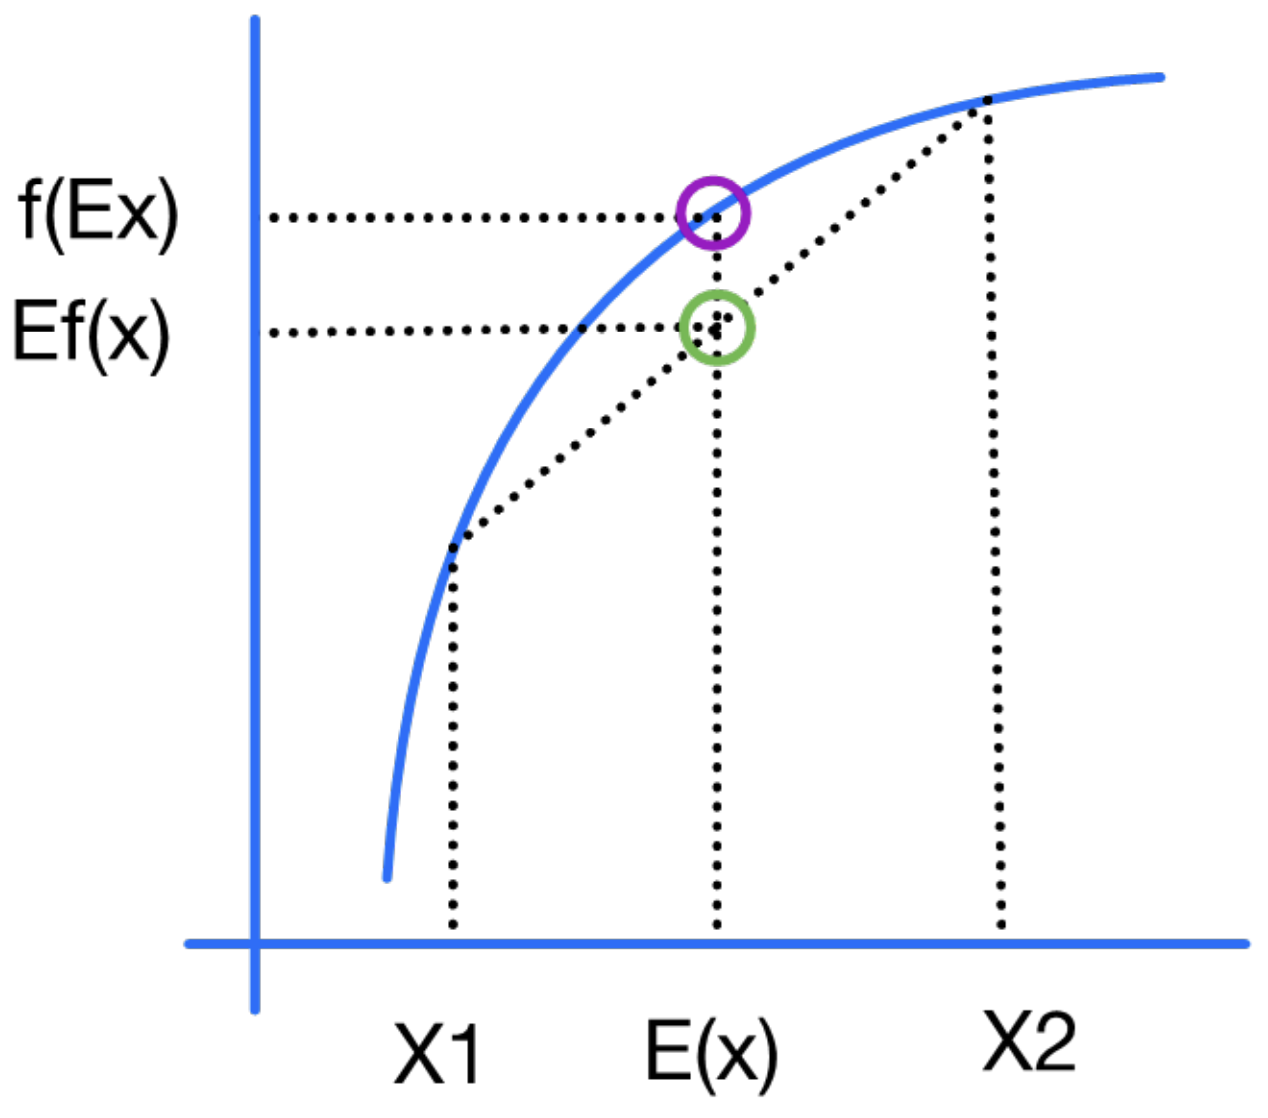
\includegraphics[width=0.50\textwidth]{fig2.png}
    \caption{Jensen's inequality: Expected utility of gamble vs. utility of expected value}
    \label{fig:fig2}
\end{figure}

The size of this risk premium depends on the investor’s risk aversion (the curvature of $u$) and on the distribution of the risky asset’s returns. To understand how large this premium must be in practice, we now turn to the empirical behavior of returns for individual securities and portfolios.
\section{Distribution of Stocks and Portfolios}

\subsection{Individual Stocks}
Investors seek to protect their portfolio, and public equities, now totaling \$51 trillion market value, plays a central role.

We simulated $500,000$ daily returns of an individual stock using the jump-diffusion model of \citet{backus2011disasters}. The model combines a smooth diffusion process, drawn from a normal distribution, with rare discontinuities: jumps whose count follows a shifted geometric distribution and whose size and direction follow a second normal distribution.

Note that stock returns are highly positively skewed. Most stocks perform poorly or modestly on most days, while a small fraction produce outsized gains. Since prices cannot fall below zero, downside is bounded, but upside remains unbounded. This asymmetry shifts the mean return above the median, unlike for a normal distribution where the mean coincides with the median. Studies support this pattern, showing that the median return on individual stocks is often below that of Treasury bills, even though on average, stocks have outperformed bonds by a factor three \citep{bessembinder2018stocks,oh2022cross}.

The parameters for this return simulation reflected the above (see Appendix~\ref{appendix:code}), while emphasizing the skewness of individual stocks. We use a moderate, positive mean return to indicate the long-run equity premium ($\mu = 0.04$), while incorporating a realistic range of fluctuations with the baseline volatility ($\sigma = 0.0324$). The dynamics that dictate variance are $\omega = 0.33$ (jump intensity) $, \theta = 0.12$ (mean jump size) $, \delta = 0.0064$ (volatility of jumps). The resulting distribution in \autoref{fig:fig3} exhibits a skewness of roughly $3$ and kurtosis of $19.8$. 


\begin{figure}[h]
    \centering
    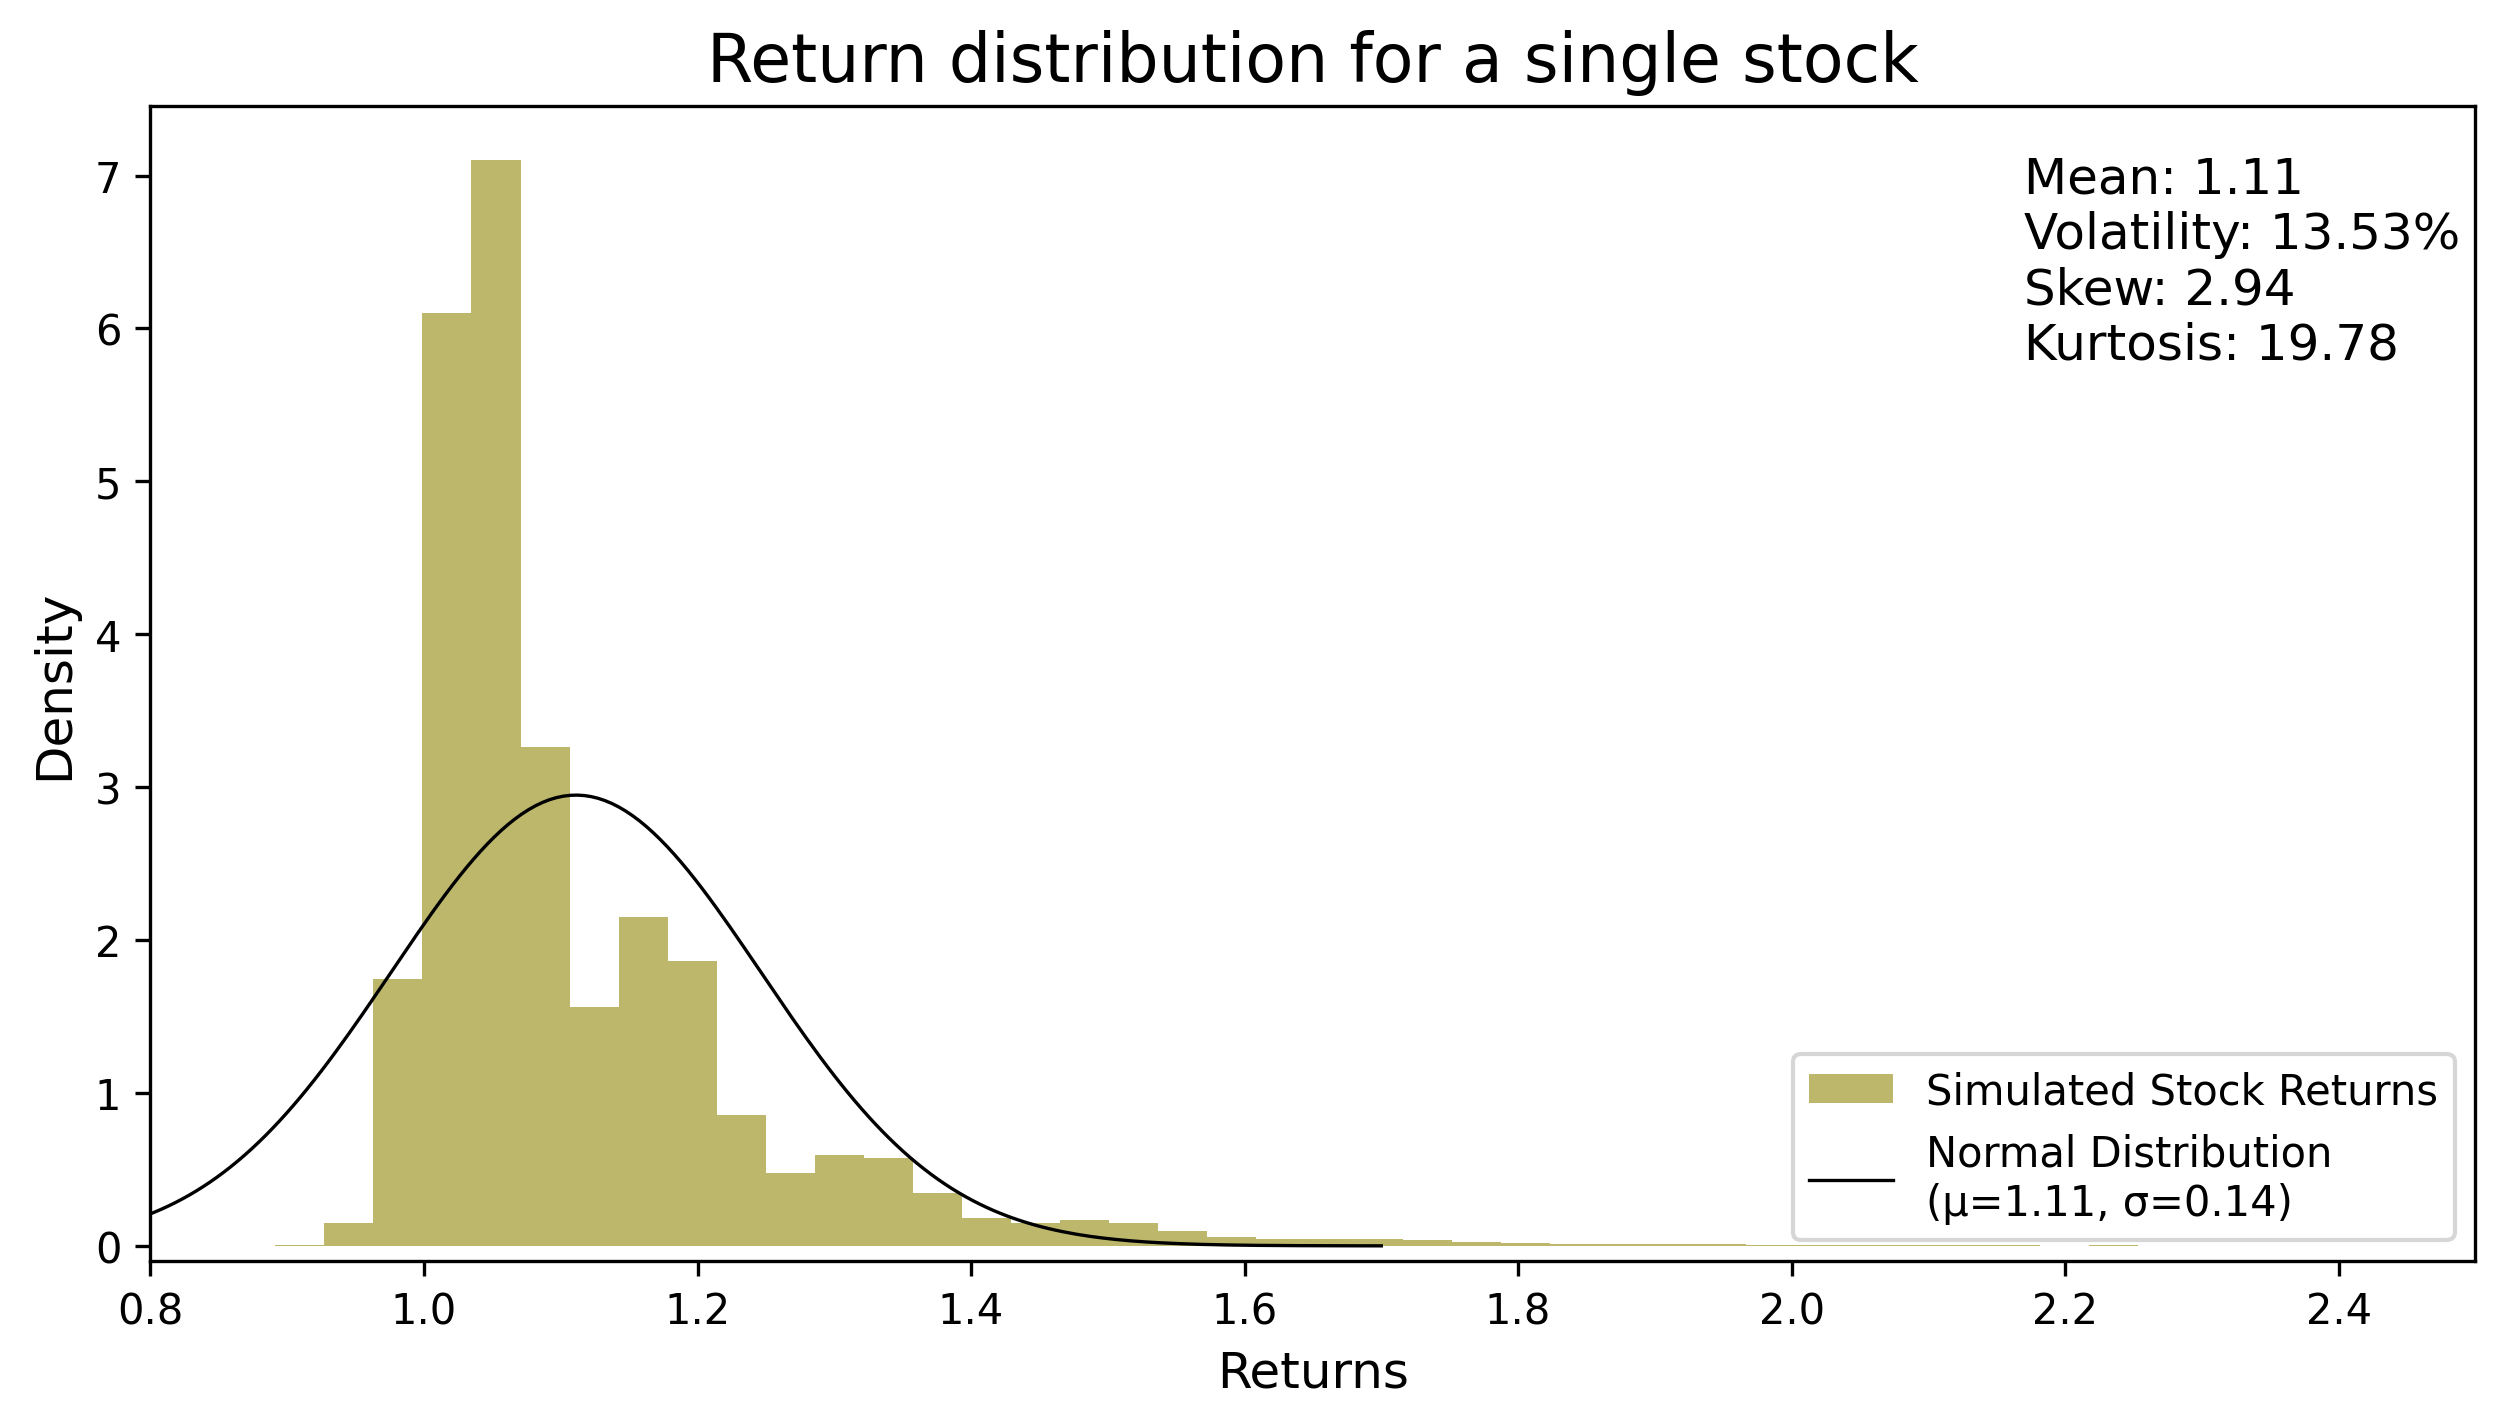
\includegraphics[width=0.75\textwidth]{fig3.png}
    \caption{Simulated return distribution for a single stock, showing strong positive skew and fat tails}
    \label{fig:fig3}
\end{figure}

The positive skew translates into the very long right tail in the distribution. Real stocks echo this pattern. Consider a company developing a new product (such as a new gene therapy treatment). The product may face a high probability of failure, yet if it succeeds, the benefits will be large. This payoff structure creates the right-skewed distribution of daily returns that appears in many small-cap biotech firms, like Sarepta Therapeutics, which exhibits a skewness of $8.49$ (\autoref{fig:fig4}). Most days produce modest or negative returns, but occasional breakthroughs, regulatory approvals, or acquisitions generate outsized gains. 
Note the extraordinarily high kurtosis in \autoref{fig:fig4}, measured at 248. This extreme value arises from a handful of outlier days with gross returns much higher than the mean (approximately $2.00, 1.46,$ and $1.03$). Such rare but very large deviations inflate the tails of the distribution, driving kurtosis upward.

Similarly, the high kurtosis in \autoref{fig:fig3} indicates that extreme events occur in individual stock returns more often than a normal model would suggest. Even a large, diversified company such as Apple displays high kurtosis (\autoref{fig:fig5}) in its daily return distribution (despite relatively low skew) because its returns still experience fat-tailed shocks. 

\begin{figure}[h]
    \centering
    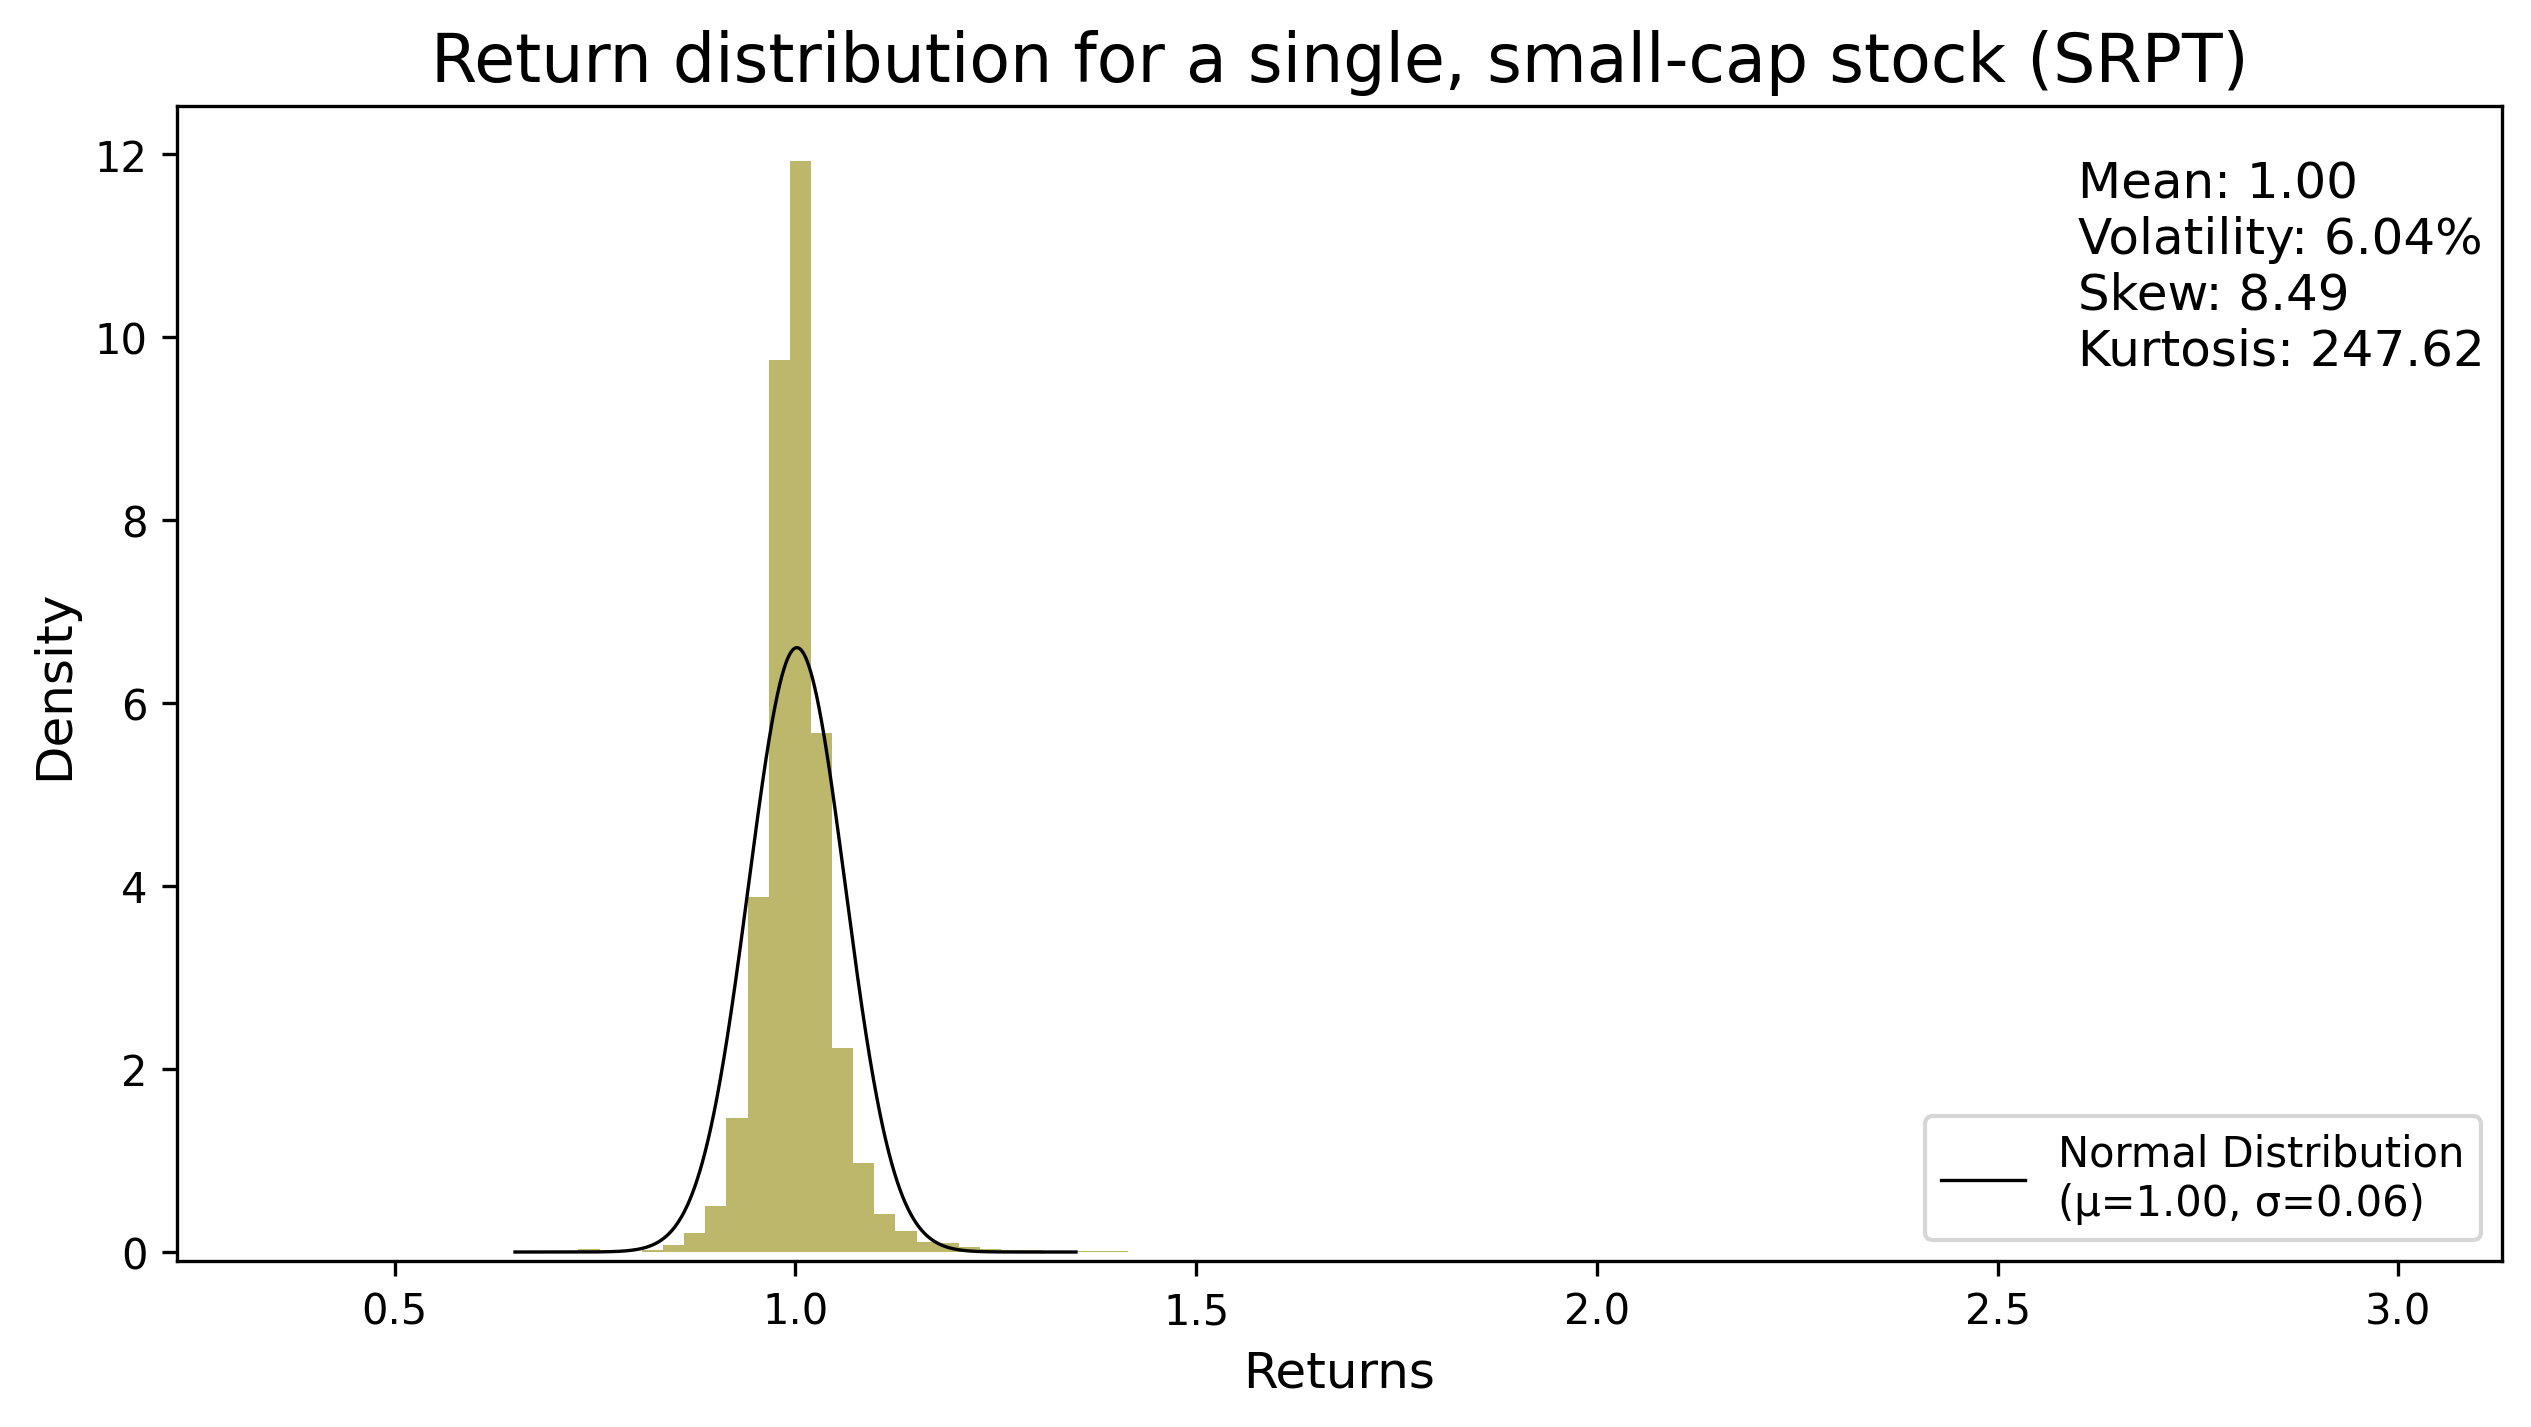
\includegraphics[width=0.75\textwidth]{fig4.png}
    \caption{Empirical return distribution of Sarepta Therapeutics}
    \label{fig:fig4}
\end{figure}

\begin{figure}[h]
    \centering
    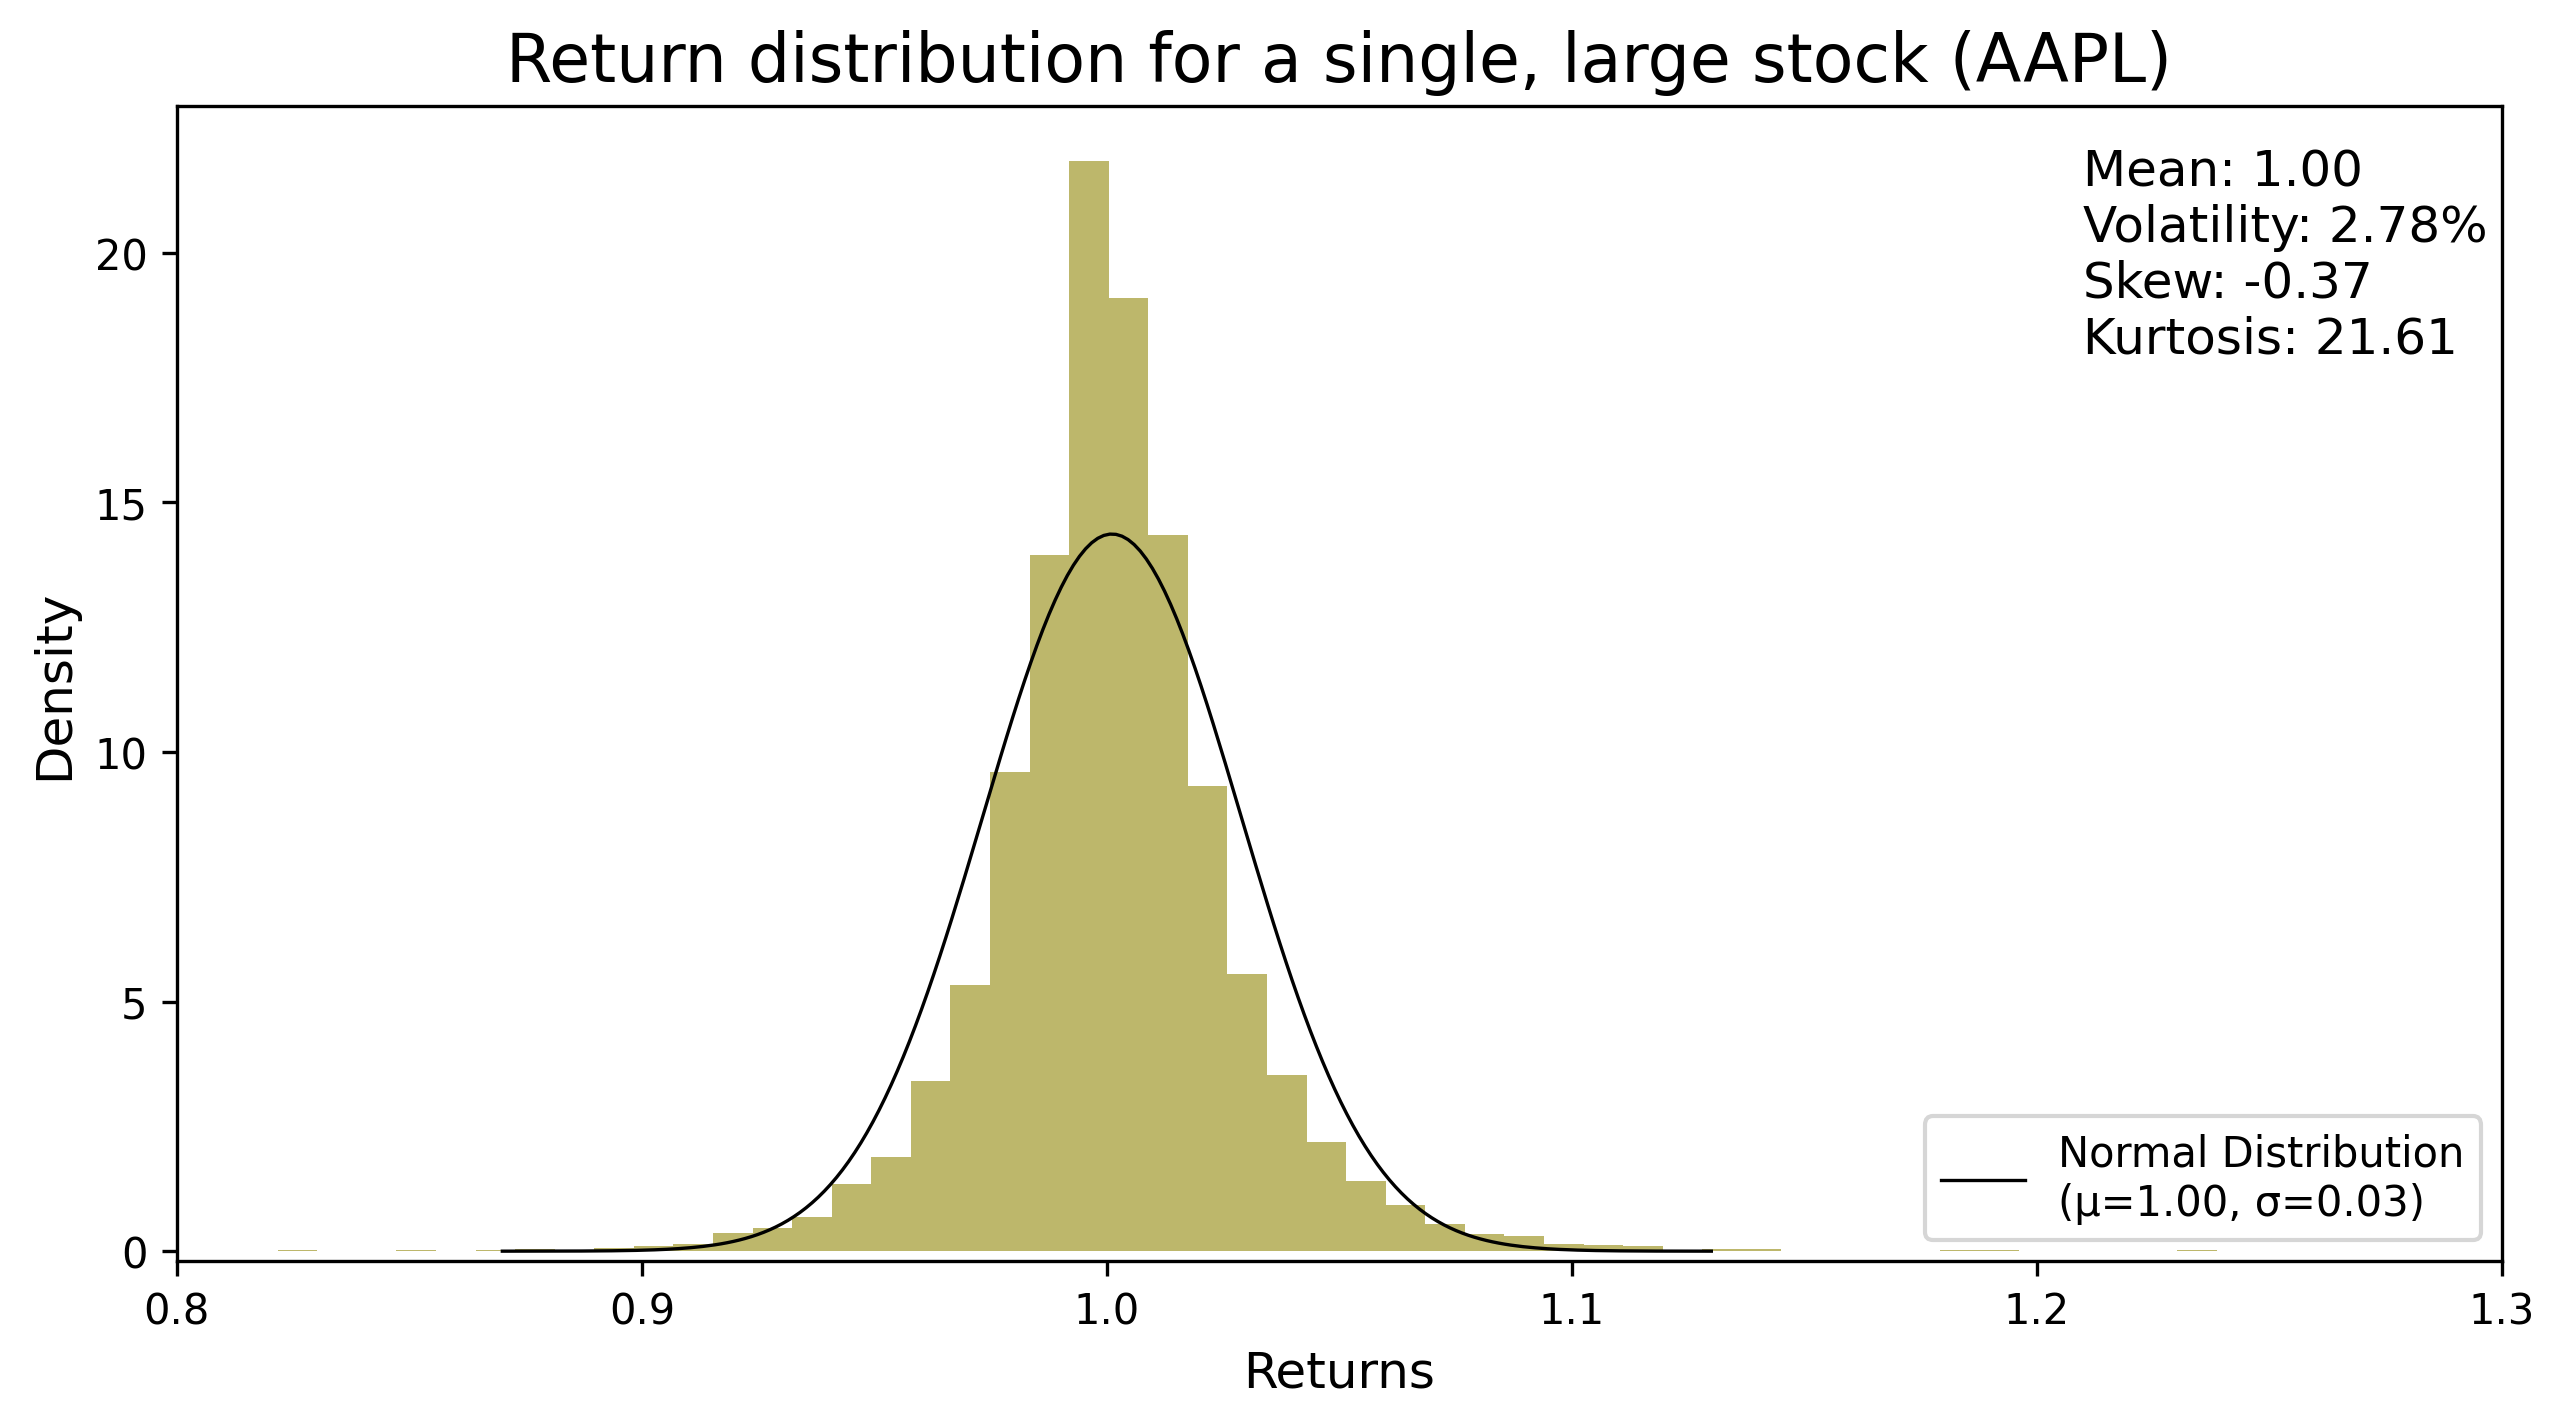
\includegraphics[width=0.75\textwidth]{fig5.png}
    \caption{Return distribution of Apple}
    \label{fig:fig5}
\end{figure}

These return distributions are risky, in that they are not well-captured by variance alone. High skew and fat tails imply that mean-variance analysis misses much of the story.

\subsection{Portfolio Returns}
The issue with individual stocks is the wild returns. However, the central limit theorem predicts that summing many independent variables results in a normal distribution. Furthermore, the law of large numbers tells us that the variance should approach zero.  

We construct a diversified portfolio by averaging 100 independent and identically distributed stocks from the model used in \autoref{fig:fig3}. Each simulated portfolio return is the mean of 100 stocks at each date $t$ (see Appendix~\ref{appendix:code}). The resulting distribution of daily returns is shown in \autoref{fig:fig6}.

\begin{figure}[h]
    \centering
    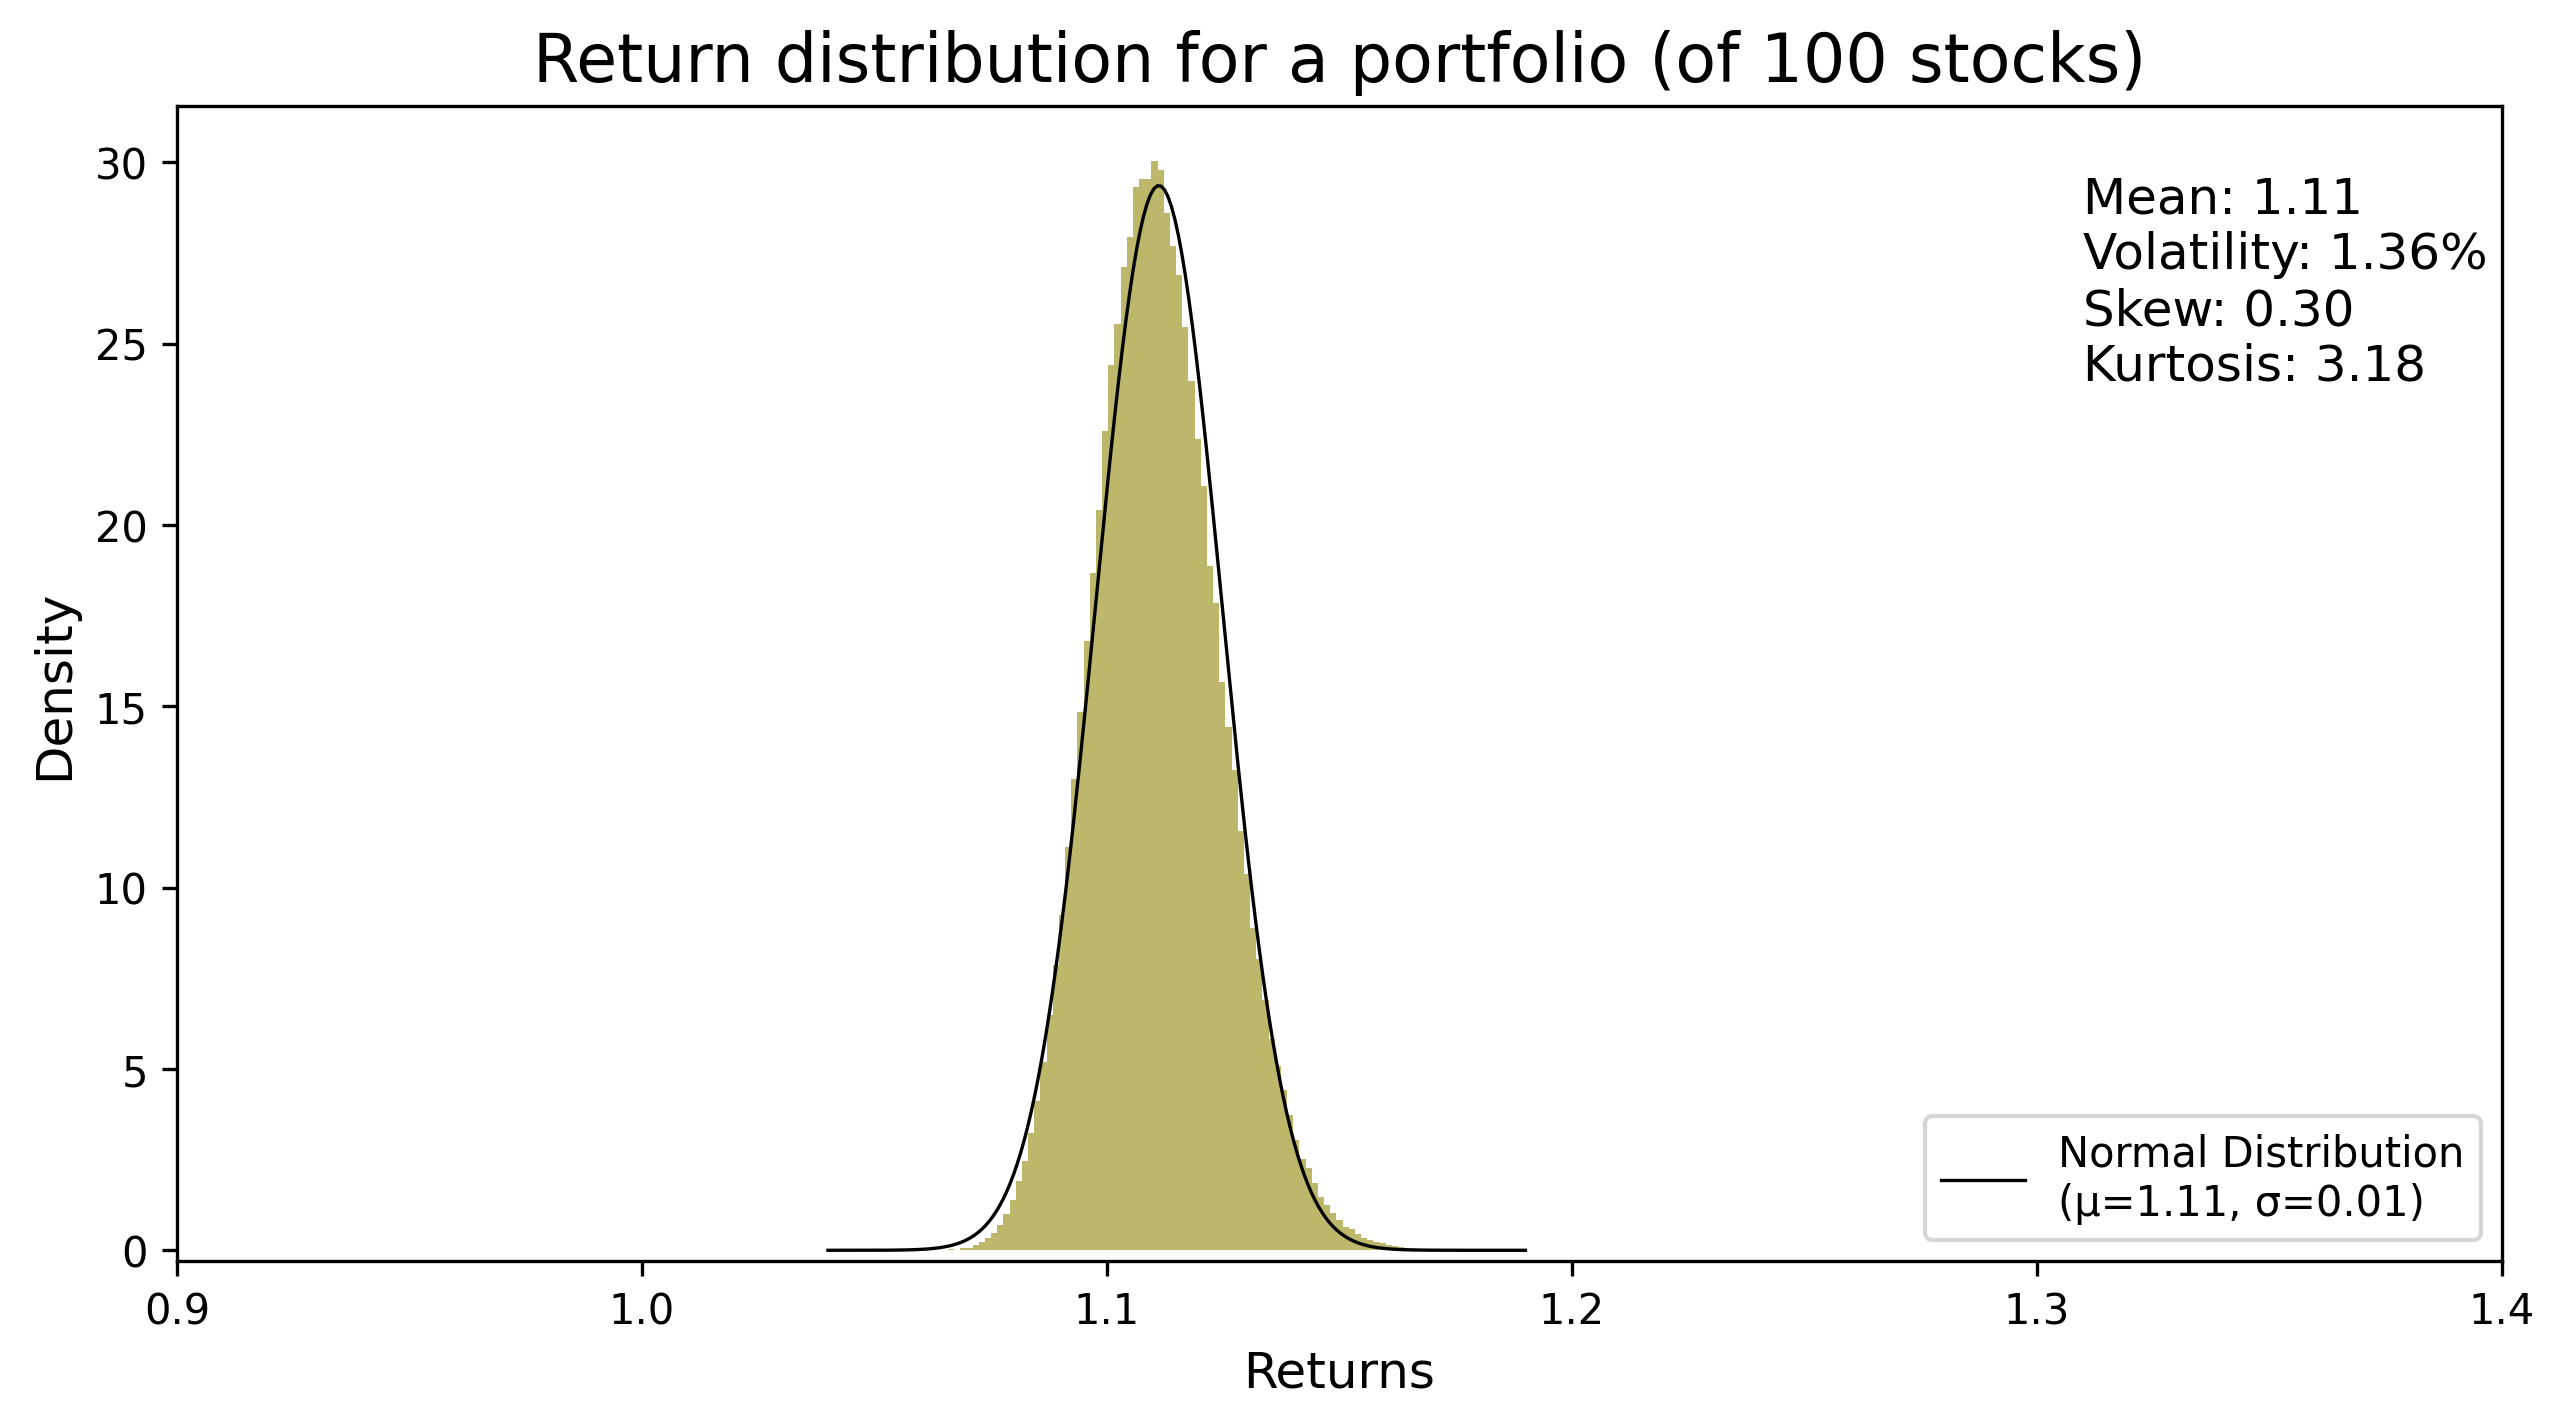
\includegraphics[width=0.75\textwidth]{fig6.png}
    \caption{Simulated portfolio daily return distribution from averaging 100 stock simulations}
    \label{fig:fig6}
\end{figure}

The portfolio shows low skew ($= 0.30$) and near-normal kurtosis ($= 3.18$). Thus, diversification removes much of the \say{unexpectedness} in individual stock returns. The fat right tails of some firms are offset by the poor returns of others, resulting in a thinner-tailed, symmetric return profile with a lower variance.

However, diversification does not eliminate risk; it transferred from undiversified investors to a wide pool of capital providers. Capital providers must trust firm managers to deploy funds responsibly. But once capital is raised, managers may bear little downside and capture most of the upside. They may shrink, take excessive risks, or divert resources toward perks. The very act of pooling capital introduces moral hazard. For diversification to work, agency problems must be solved.
\section{Moral Hazards}

\subsection{A Simple Model for a Moral Hazard}

A moral hazard occurs when capital providers cannot monitor the actions of an agent who controls funds and may extract value. For example, a \say{too-big-to-fail} bank might pursue tail-risk trades, knowing deposit insurance limits its downside. 

We analyze a canonical model of entrepreneurial effort and financing constraints, adapted from \citet{holmstrom2011inside} and summarized in \autoref{fig:fig7}.

\begin{figure}[h]
    \centering
    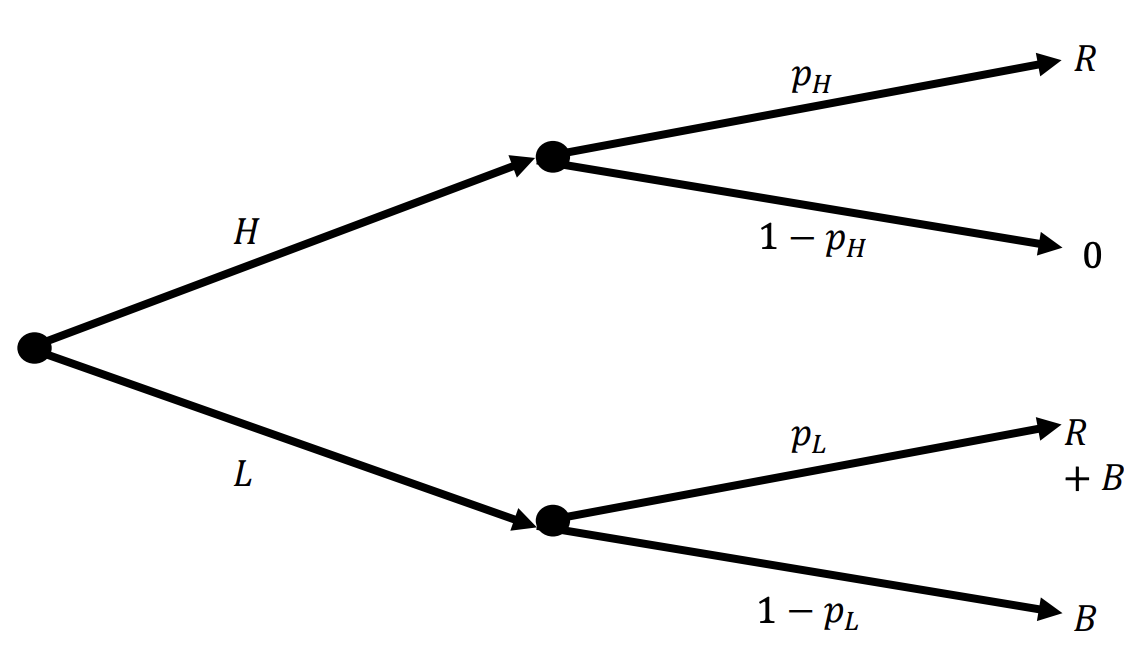
\includegraphics[width=0.75\textwidth]{fig7.png}
    \caption{Financing constraint under moral hazard}
    \label{fig:fig7}
\end{figure}

Consider a single entrepreneur who requires outside investment of $I$ to launch a project that will pay $R$ upon success but nothing upon failure. When the entrepreneur works hard (the high-effort choice), the project succeeds with probability $p_H$. Conversely, shrinking to a low-effort level lowers the success probability to $p_L$, where $p_L < p_H$ but allows the entrepreneur to get a private benefit of $B$ (i.e., perks or diverted cash) assumed to be certain. We assume the following conditions:
\begin{itemize}
    \item The project is socially efficient: $p_H R > I$
    \item Private benefit is not so large that it outweighs the high-effort surplus, due to decreasing marginal utility and how companies often succeed in creating wealth for large dispersed shareholders: $B< p_H R$
    \item Investors would still break even if the entrepreneur shirks: $I < p_L R$
\end{itemize}

The risk arises because investors cannot observe effort directly, so they must design a contract that makes high effort preferable. Let the contract promise the entrepreneur $X_s (\ge 0)$ if the project succeeds and $X_f$ if it fails. For high effort to dominate low effort, the entrepreneur's expected payoff from exerting effort must weakly exceed the payoff from shirking:
\[
p_H (R - X_s) + (1 - p_H) X_f \geq p_L (R - X_s) + (1 - p_L) X_f + B
\]

Subtracting both sides yields:
\[
X_s - X_f \geq \frac{B}{\Delta p}
\quad \text{where } \Delta p = p_H - p_L
\]


Since limited liability prevents investors from charging the entrepreneur money after a failure, we can assume $X_f = 0$. Thus, the minimum success-state payment is $X_s^{min} = \frac{B}{\Delta p}$. Note that every dollar committed to $X_s^{min}$ is a dollar that cannot be pledged to investors. Every dollar allocated to $X_s^{min}$ cuts the cash flow investors can claim; thus, the largest expected cash-flow is $p_H(R- \frac{B}{\Delta p})$.

Financing this project is only feasible if the required capital $I$ does not exceed this amount. If $I> p_H(R- \frac{B}{\Delta p})$, no contract can keep both the entrepreneur honest and allow investors to break even, so the project would die in the fund-raising stage.

Note the restrictions of the model, as it distills the distribution of returns from \autoref{fig:fig6} into binary outcomes: success or failure. Moreover, the multiple ways an entrepreneur can influence a project for better or worse are also collapsed into choices labeled “high” and “low” effort.


\subsection{How Market Regulation Can Help}
Market regulation can ease the moral‑hazard financing constraint by shrinking the entrepreneur’s private benefit $B$ or raising $\Delta p$. Rules regarding insider trading and limits on related-party transactions directly reduce $B$. Mandatory disclosure and continuous reporting improve monitoring, so low effort is more likely to be detected and prevented, raising $\Delta p$. 

Though this may seem to make things worse for the entrepreneur because a private benefit is going away, the entrepreneur would far rather receive a share of profits from a successful venture than not be able to finance a venture at all. By expanding the set of projects that attract funding and protecting outside money, well‑designed regulation is therefore Pareto‑improving: it benefits both entrepreneurs and investors through efficient capital allocation \citep{holmstrom2011inside}.

In doing so, regulation makes broad-based risk-sharing (i.e., modern equity markets) feasible at scale.
\section{Aggregate Market Returns}

\subsection{Daily Returns on the Market Portfolio}
In \autoref{fig:fig6}, we modeled a diversified portfolio, showing that aggregation reduced skewness and kurtosis of an individual stock. 

We now turn to real daily market returns. \autoref{fig:fig8} shows daily returns from a value-weighted market portfolio (sourced from CRSP, 6/1/1988-12/31/2022), excluding ADRs and adjusting for dividends. The three most extreme downside return days occurred on 10/15/2008, 03/12/2020, and 03/16/2020 (WRDS query and code provided in Appendix ~\ref{appendix:code}). 

\begin{figure}[h]
    \centering
    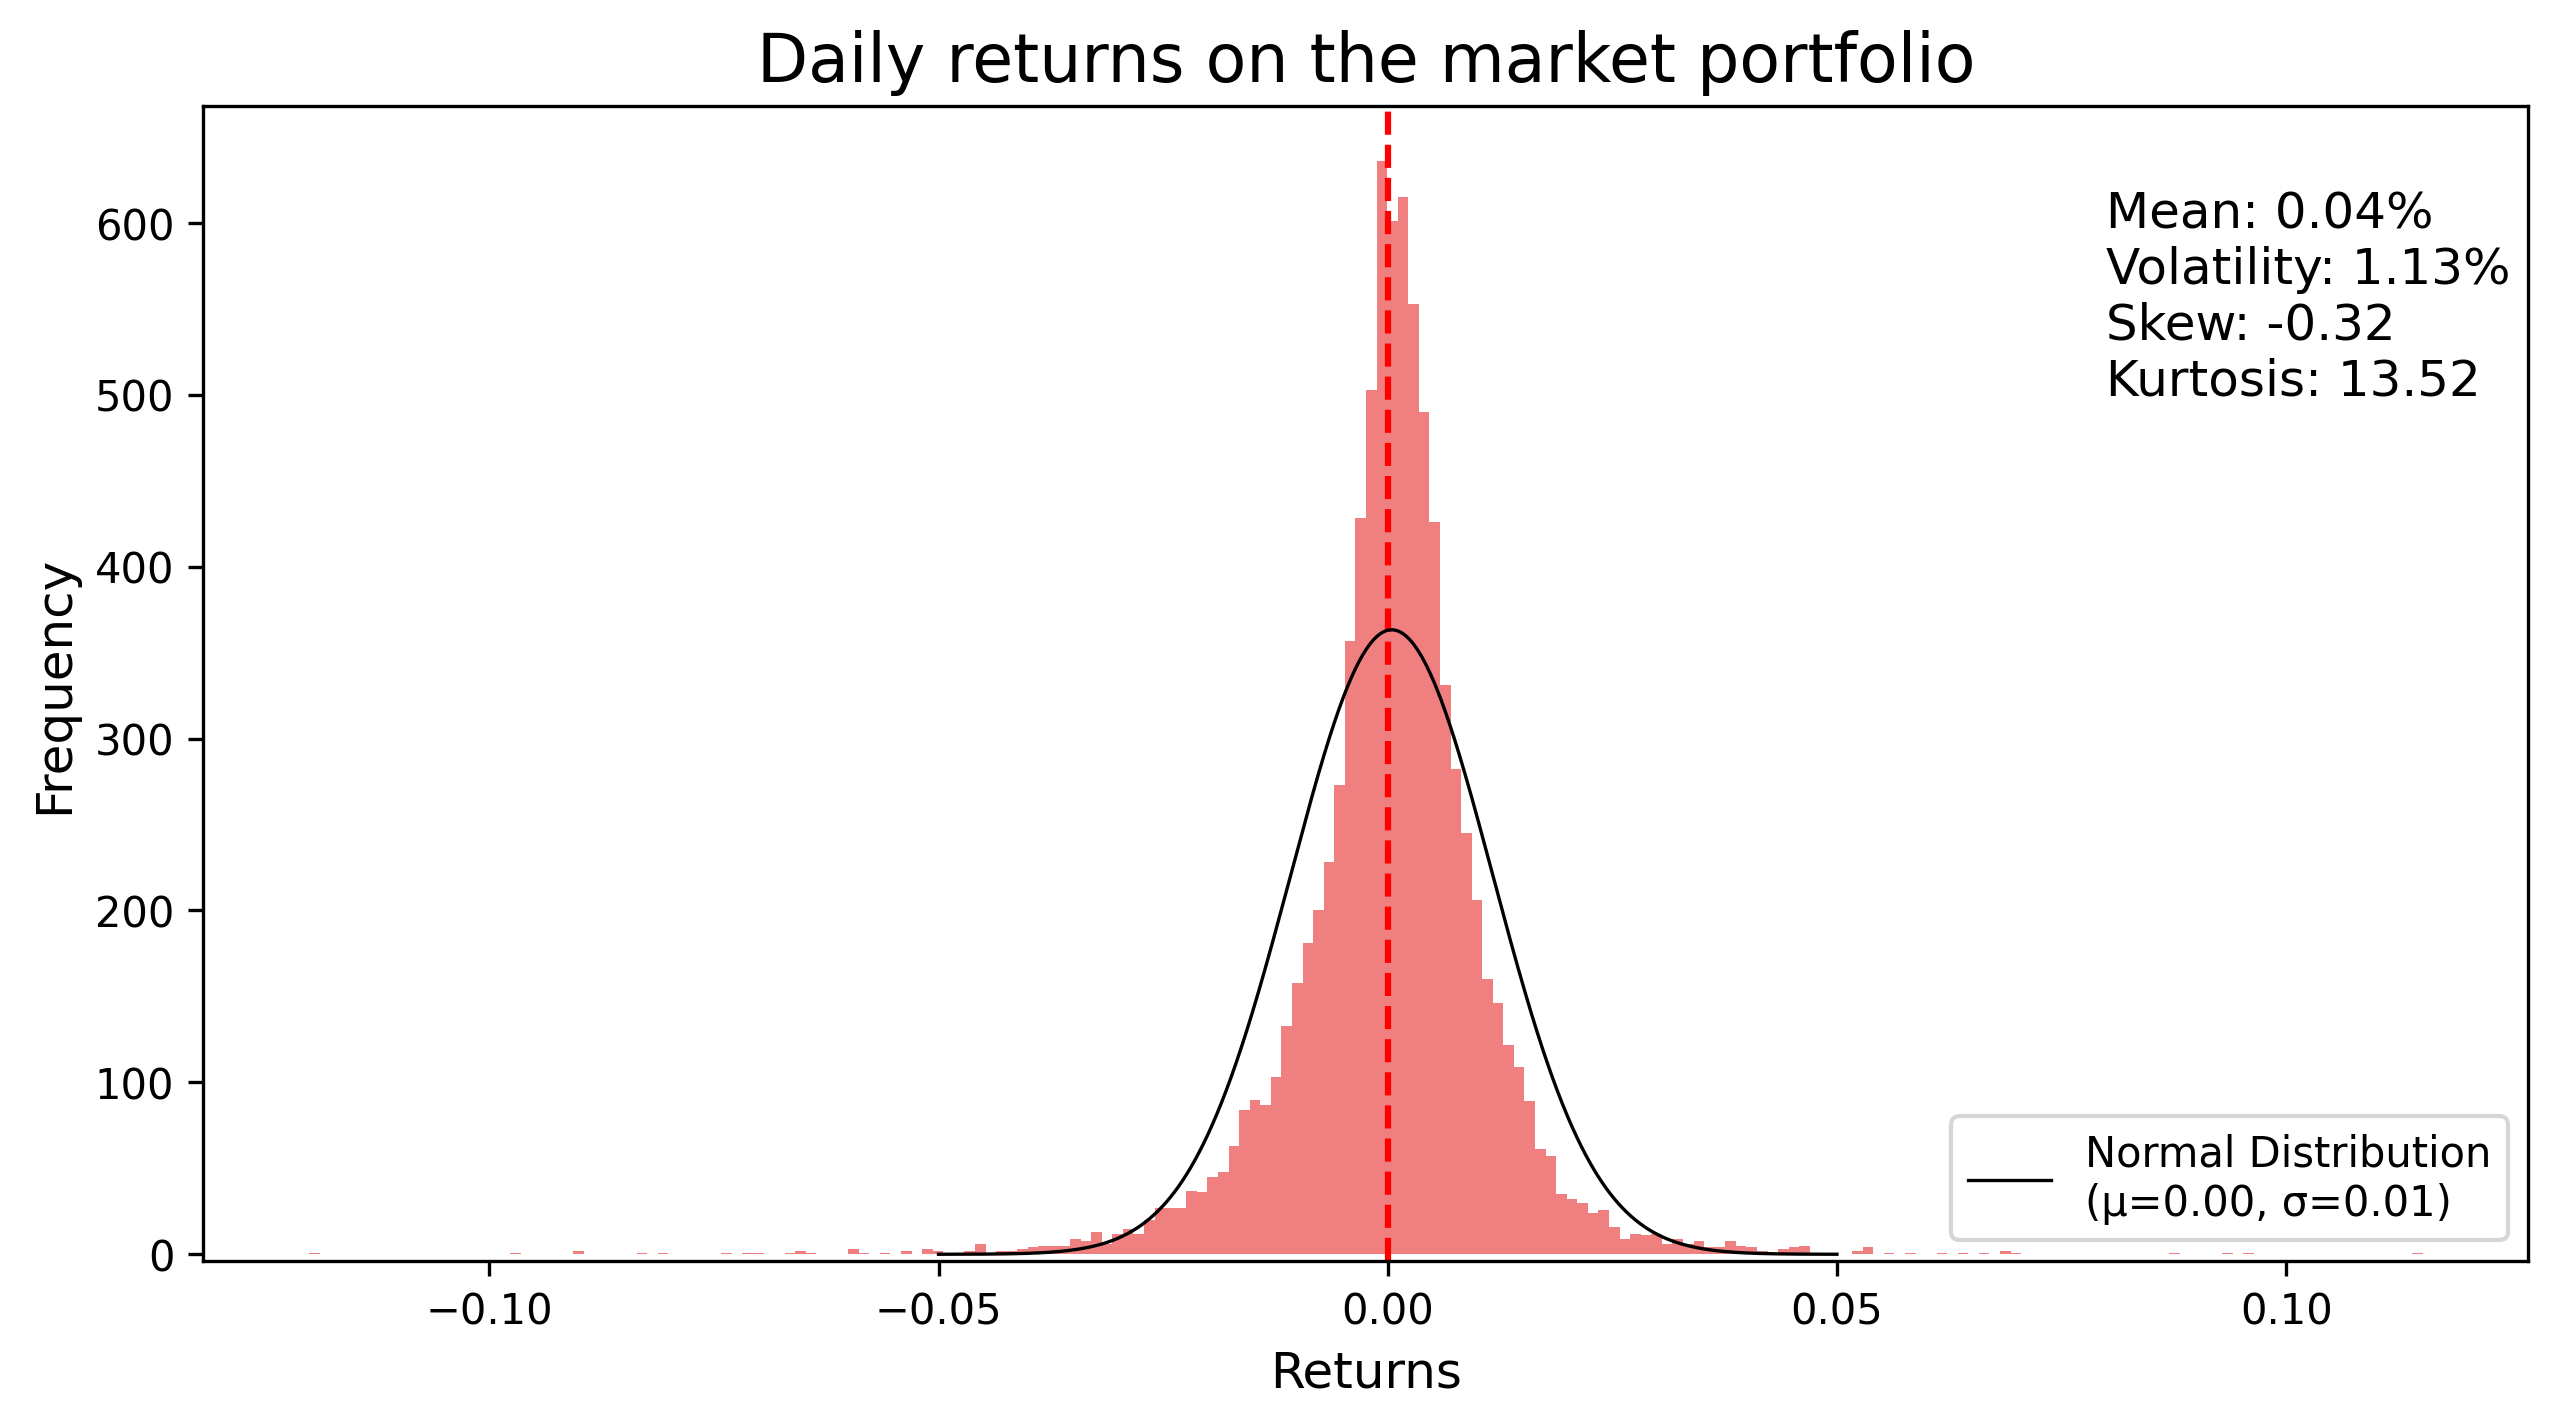
\includegraphics[width=0.75\textwidth]{fig8.png}
    \caption{Distribution of daily returns for the CRSP market portfolio (1988–2022)}
    \label{fig:fig8}
\end{figure}

The data reveal a daily mean return of 0.04\%, a standard deviation of 1.13\%, skewness of –0.32, and kurtosis of approximately 14. A daily return of 0.04\% translates into an average annual return of $0.04 \cdot 250 =  10\%$, while a daily volatility of 1.13\% translates into an annual volatility of $1.13 \cdot \sqrt{250} \approx 17.9\%$.

Unsurprisingly, aggregate returns exhibit negative skewness even though individual stocks often display positive skewness. Idiosyncratic good news (a drug approval, a tech breakthrough) lifts single-firm performance but diversifies away in the index, while broad negative news (macro shocks, liquidity freezes) affects many firms simultaneously, producing a heavier downside tail. Yet, regulations have promoted fairness, orderliness, and efficiency in markets when volatility spikes. In that sense, high volatility markets repeatedly remind investors to “expect the unexpected”.

However, there is one aspect of the unexpected that is notoriously hard to detect. Note that the kurtosis is roughly 14. Kurtosis has a problem that the mean does not have, and the variance has to a much lesser degree: it is biased downwards.

\subsection{Hidden Kurtosis}
Sample kurtosis is supposed to measure the fat tails of a distribution. However, true kurtosis may be much larger than any one sample indicates. 

To test this bias, we simulated $500,000$ market returns using the jump-diffusion model from Section 2, calibrated with the parameter set that \citet{backus2011disasters} link to heavy‐tailed behavior to achieve the high kurtosis and negative skewness associated with market returns (parameters specified in Appendix ~\ref{appendix:code}). We then computed the population kurtosis of this simulated distribution.

To illustrate how sample estimates understate true tail risk, we conducted a Monte Carlo experiment: we took $10,000$ independent random samples of $50$ randomly selected returns each (without replacement) from the simulated population and calculated the sample kurtosis for each draw. \autoref{fig:fig9} shows the distribution of the $10,000$ sample estimates of kurtosis. To obtain an average sample kurtosis of $15$, we need a population kurtosis of over 100.

\begin{figure}[h]
    \centering
    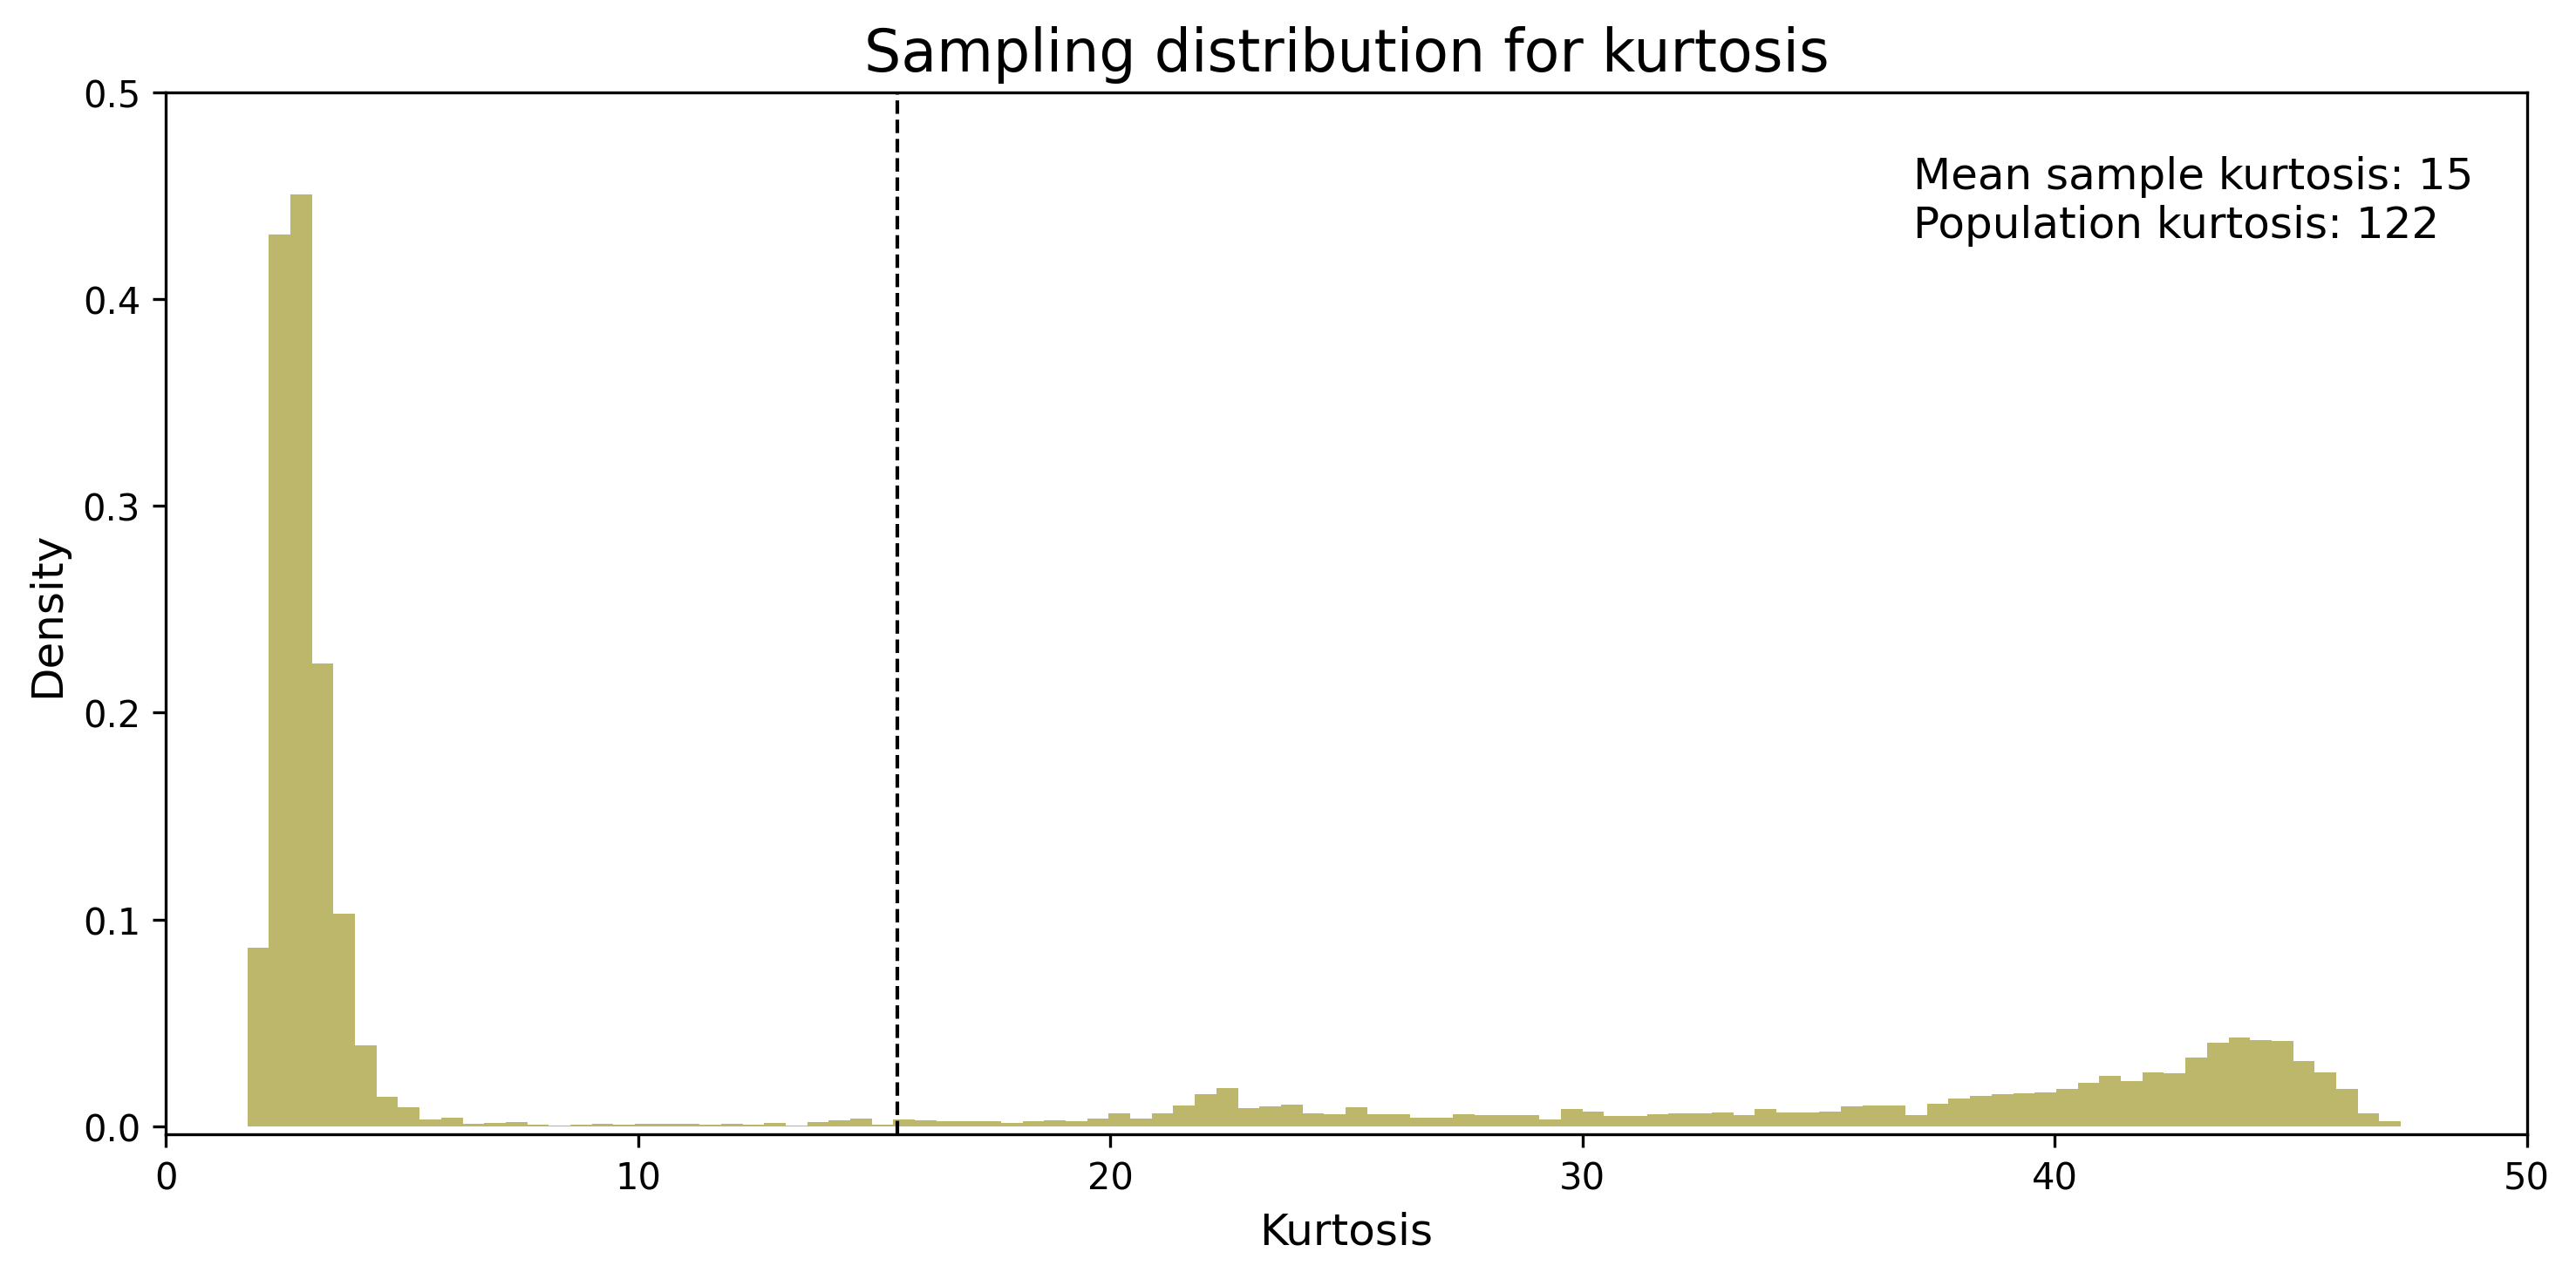
\includegraphics[width=0.75\textwidth]{fig9.png}
    \caption{Distribution of sample kurtosis, where true kurtosis exceeds 100}
    \label{fig:fig9}
\end{figure}

Intuitively, rare events will always catch markets off guard, so it is tempting to lean on statistics such as sample kurtosis for reassurance about tail risk. Yet our simulation shows that even when the true kurtosis exceeds 100, most 50‑day samples report values well below 15. Because small samples almost always understate true kurtosis, they can only tell us that returns are not normal, never that they are safely close to normal. Accurately gauging those fat tails is therefore critical for securities whose pay‑offs are highly sensitive to extreme moves, since underestimating kurtosis means underestimating the probability and cost of rare, severe shocks.
\section{Options and Tail Risk}

A particularly interesting example of tail risk comes from put options on market indices, whose payoffs make tail risk and potential mispricing visible at a glance. 

\subsection{Options Background}
A put option gives the holder the right to sell a security for a fixed amount, $K$ (the exercise/strike price). \autoref{fig:fig10}(a) shows the payoff for buying (or going long) a put option at maturity as a function of the price of the underlying security at expiry, $S_1$. Conversely, \autoref{fig:fig10}(b) shows the other side of the options contract (i.e., writing or shorting a put option). 

\begin{figure}[h]
    \centering
    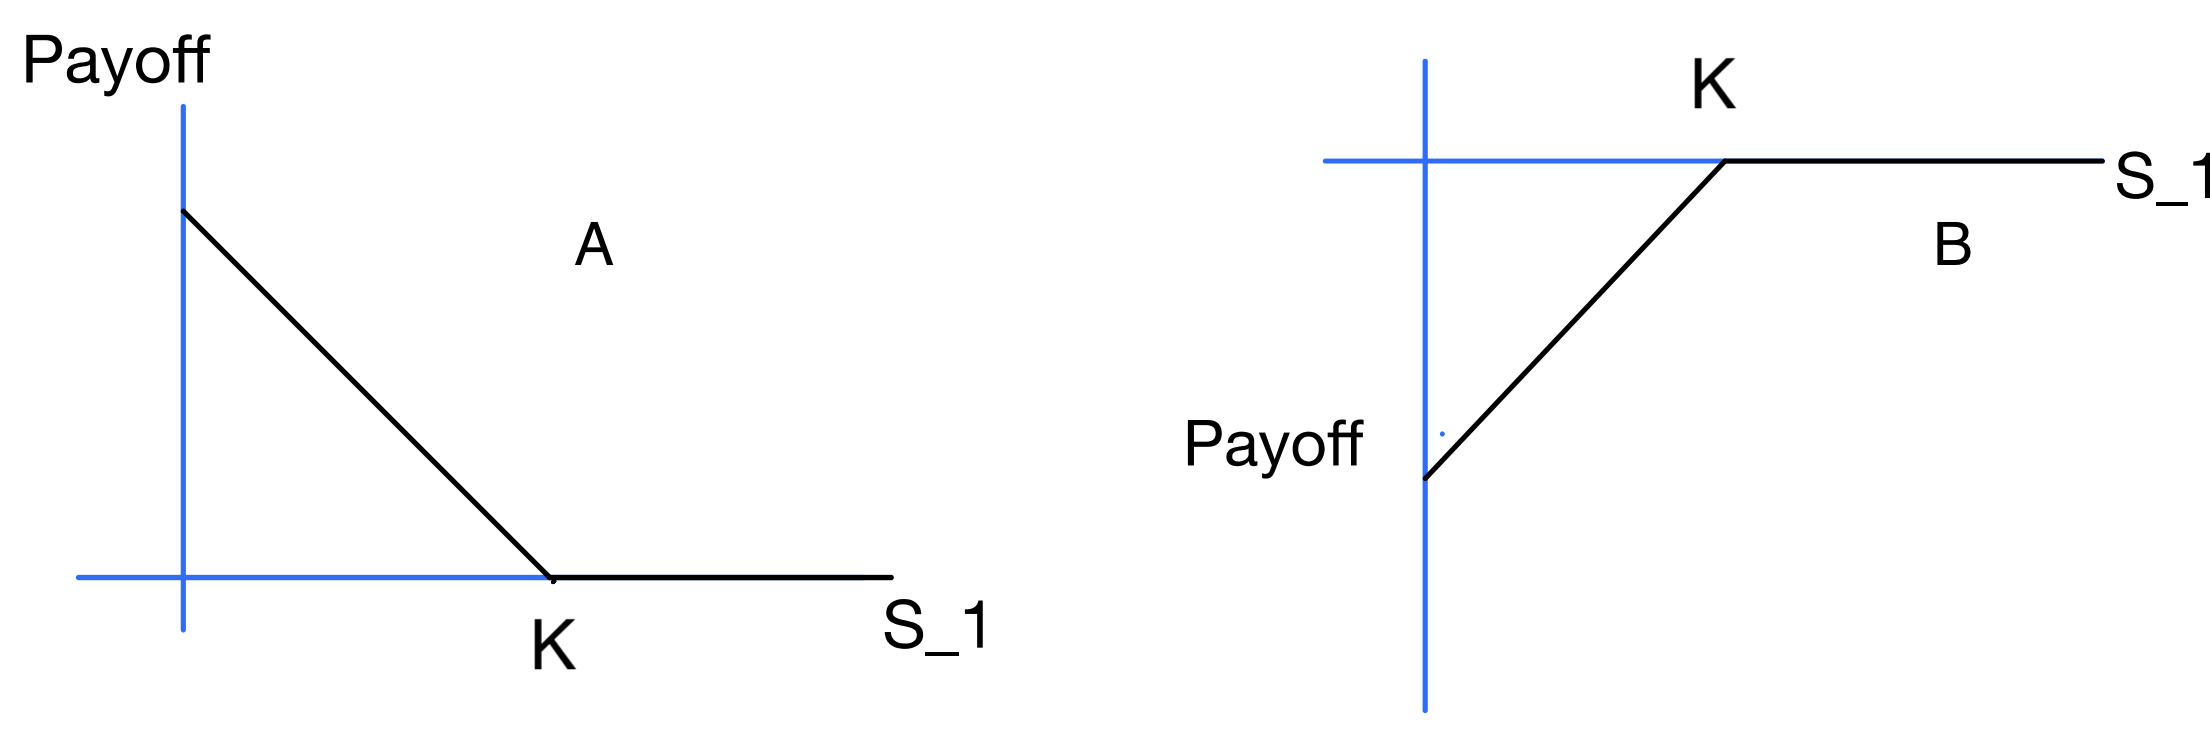
\includegraphics[width=0.50\textwidth]{fig10.png}
    \caption{Payoffs for long and short put options}
    \label{fig:fig10}
\end{figure}

The payoff for buying a put option is $max(K - S_1, 0)$. When $S_1 \ge K$, the option is considered out-of-the-money (OTM). The payoff of an OTM put is $0$ because one would not exercise the option. When $S_1 < K$, the option is considered in-the-money. The payoff for the buyer is $K-S_1$, and the writer of the option is forced to buy the security for more than it is worth. Thus, the put option’s seller insures the buyer against the underlying’s price decline. 

This payoff structure introduces negative skewness for the writer. Most of the time ($S_1 \ge K$), the writer will pay out zero, whereas only some of the time ($S_1 < K$) the writer will pay out something positive. Because of this negative skew, the writer of the option earns a \say{premium} ($p$), the positive amount that the options buyer pays. Thus, when writing puts on broad market indices, the strategy initially appears attractive since large market crashes are relatively rare events. The actual payoff for a put option writer is $- max(K-S_1, 0) + p$. While this sounds promising because the writer earns $p$ most of the time, the market can sometimes crash (i.e., $S_1 << K$), leading to significant losses for the writer.

The Black-Scholes model (BSM), initially published in 1973, provides a framework to determine the fair value of this premium $p$ \citep{black1973pricing}. The core of the model is a simple binomial tree (\autoref{fig:fig11}). As one holds the the maturity of an option constant and increases the number of steps within the binomial tree, by the central limit theorem, the distribution of returns approaches a lognormal one \citep{cox1979option}.

\begin{figure}[h]
    \centering
    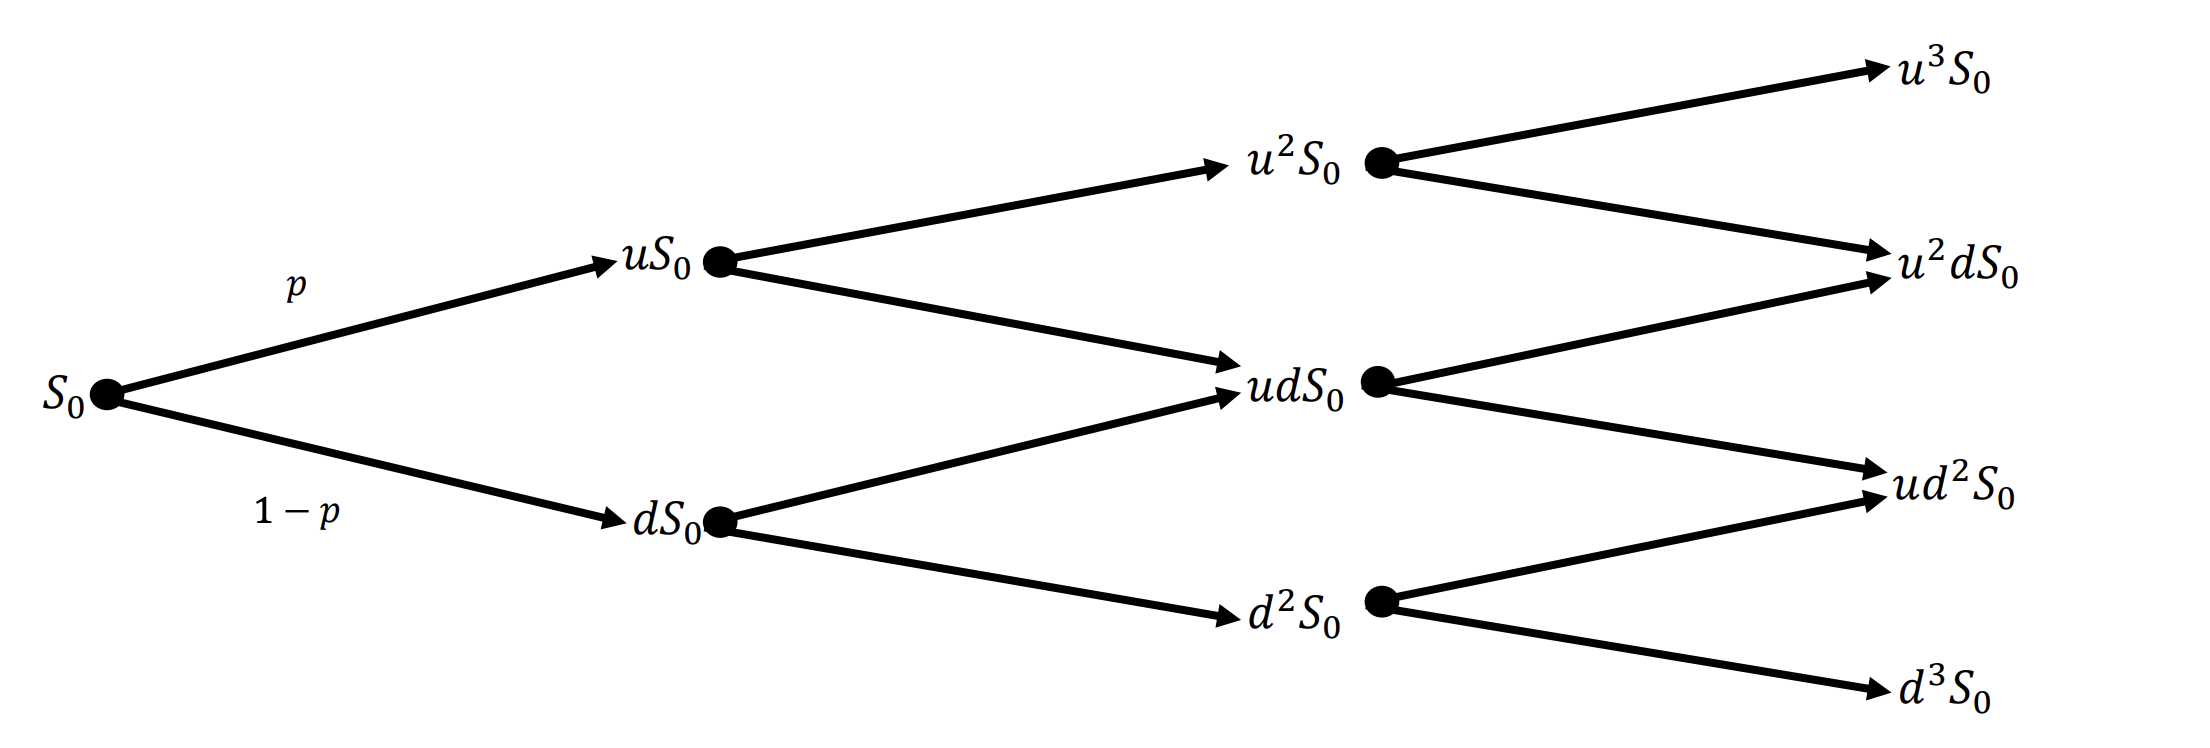
\includegraphics[width=0.75\textwidth]{fig11.png}
    \caption{Binomial tree}
    \label{fig:fig11}
\end{figure}

Black, Scholes, and Merton showed that the price of the option depends on the current value of the underlying ($S_0$; also known as spot price), exercise price ($K$), time to maturity, interest rate (risk-free rate), and volatility \citep{black1973pricing, merton1971theory}. All are directly observable except the volatility. Given an actual option price, it is possible to back out the volatility (called “implied volatility”). Since actual option prices reflect market participants’ expectation and risk preferences, this implied volatility is the market’s risk-neutral expectation of future price volatility.

If the market priced options as if the lognormal distribution were true, then implied volatility would match realized volatility, and as such, would not differ between options of different strike prices. In the initial years following the model’s publication, empirical evidence largely supported this theoretical prediction. However, the market crash of October 19, 1987, marked a structural deviation. 


\subsection{The 1987 Crash}
\autoref{fig:fig12}(a) \citep{benzoni2011explaining} shows the time series of the difference between implied volatility for at-the-money (ATM) and OTM 1-month put options. Specifically, this measures ${IV}_{10\% OTM} - {IV}_{ATM}$, where the OTM put has a strike price $10\%$ below the current underlying price ($K = 0.90 \cdot S_0$).

\begin{figure}[h]
    \centering
    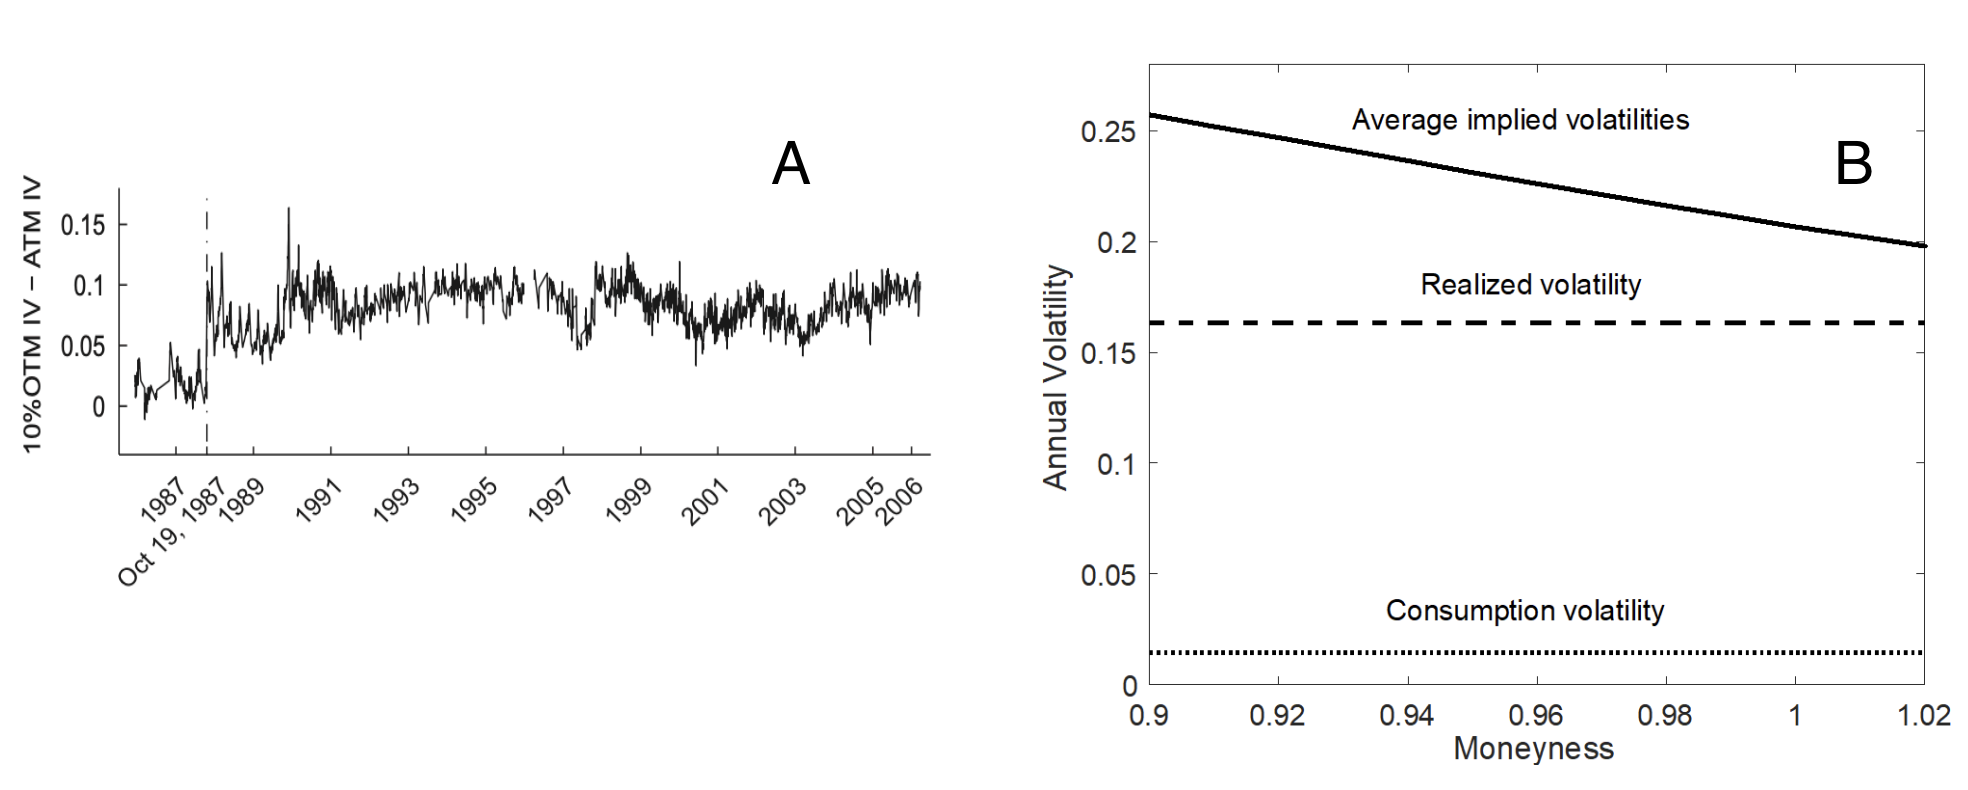
\includegraphics[width=0.75\textwidth]{fig12.png}
    \caption{Volatility skew before and after 1987 \citep{benzoni2011explaining, seo2019option}}
    \label{fig:fig12}
\end{figure}

Before October 19, 1987, the spread fluctuated around zero, indicating a flat implied volatility surface across all strikes consistent with BSM’s lognormal assumption. However, following the crash, the spread widened out and has remained wide to this day, showing that investors have since paid an ever-larger volatility premium for downside insurance.

What made October 19, 1987 so significant? The daily returns implied a 20 standard deviation event under the normal distribution assumption. To put this in perspective, the chance of an event beyond ten standard deviations is less than ${10}^{-30}$\textemdash an unimaginably small number. In the world of continuous diffusion processes underlying BSM, such an event has zero probability. For finance specialists, this meant that the supposedly arbitrage-free Black-Scholes model actually contained arbitrage opportunities after all.

This crash revealed a fundamental problem: model risk. In 1987, options traders discovered that they were using an incorrect model. This exposes two types of uncertainty. One is internal to the model, such as extreme but still-possible paths in a binomial tree. The other lies outside the model’s domain—events that the model cannot imagine. The 1987 crash was clearly the latter.

\autoref{fig:fig12}(b) \citep{seo2019option} shows how the market adapted post-crash. The figure displays average implied volatility for one-month index options as a function of \say{moneyness} (defined as the strike-to-spot ratio, $\frac{K}{S_0}$). When $\frac{K}{S_0} < 1$, the put is OTM. The downward-sloping curve shows that deeper OTM puts carry increasingly higher implied volatilities. 

This pattern reflects investors' willingness to pay higher "insurance premiums" for protection against large losses. Post-1987, the market assigns greater probability to extreme downward moves than a lognormal distribution would predict. The volatility skew has become a direct measure of tail risk concern, showing that investors now systematically overprice downside protection relative to BSM's theoretical predictions.

Why did market participants fail to incorporate tail risk into option pricing despite historical precedent? The 1929 crash (almost exactly 58 years prior to the 1987 crash) provided clear evidence against normality, yet it was largely ignored. Perhaps the $1980s$ marked the beginning of widespread quantitative modeling in finance (coming soon after BSM's publication) when practitioners had limited historical data and may have suffered from small sample bias in estimating tail probabilities.

\subsection{The Chicken Problem}
Some types of uncertainty and distributions (like the short put strategy and those with fat tails) seem destined to fool us. 

Bertrand Russell observed, \say{The man who has fed the chicken every day throughout its life at last wrings its neck instead, showing that more refined views as to the uniformity of nature would have been useful to the chicken} \citep{russell1912induction}. Bertrand Russell’s chicken is often used to invoke the failure of empiricism and inductivism. The chicken is not helped at all by having a long time series of observations. 

Writing put options exemplifies this chicken problem well. \autoref{fig:fig13} compares daily returns from the market portfolio (discussed in Section $4.1$) and a put-write strategy using CBOE data. Data on the put-writing strategy was collected from CBOE's S\&P 500 PutWrite Index, which tracks a hypothetical portfolio combining Treasury bills with short positions in at-the-money S\&P 500 put options \citep{Cboe}.

\autoref{fig:fig13} displays the stock‑market data in red, the unlevered short‑put strategy in blue, and their overlap in purple. The put-write strategy return has a similar mean but a much smaller variance and is highly concentrated at its mean. The many positive, low volatility returns can lure investors into believing in safety. 

\begin{figure}[h]
    \centering
    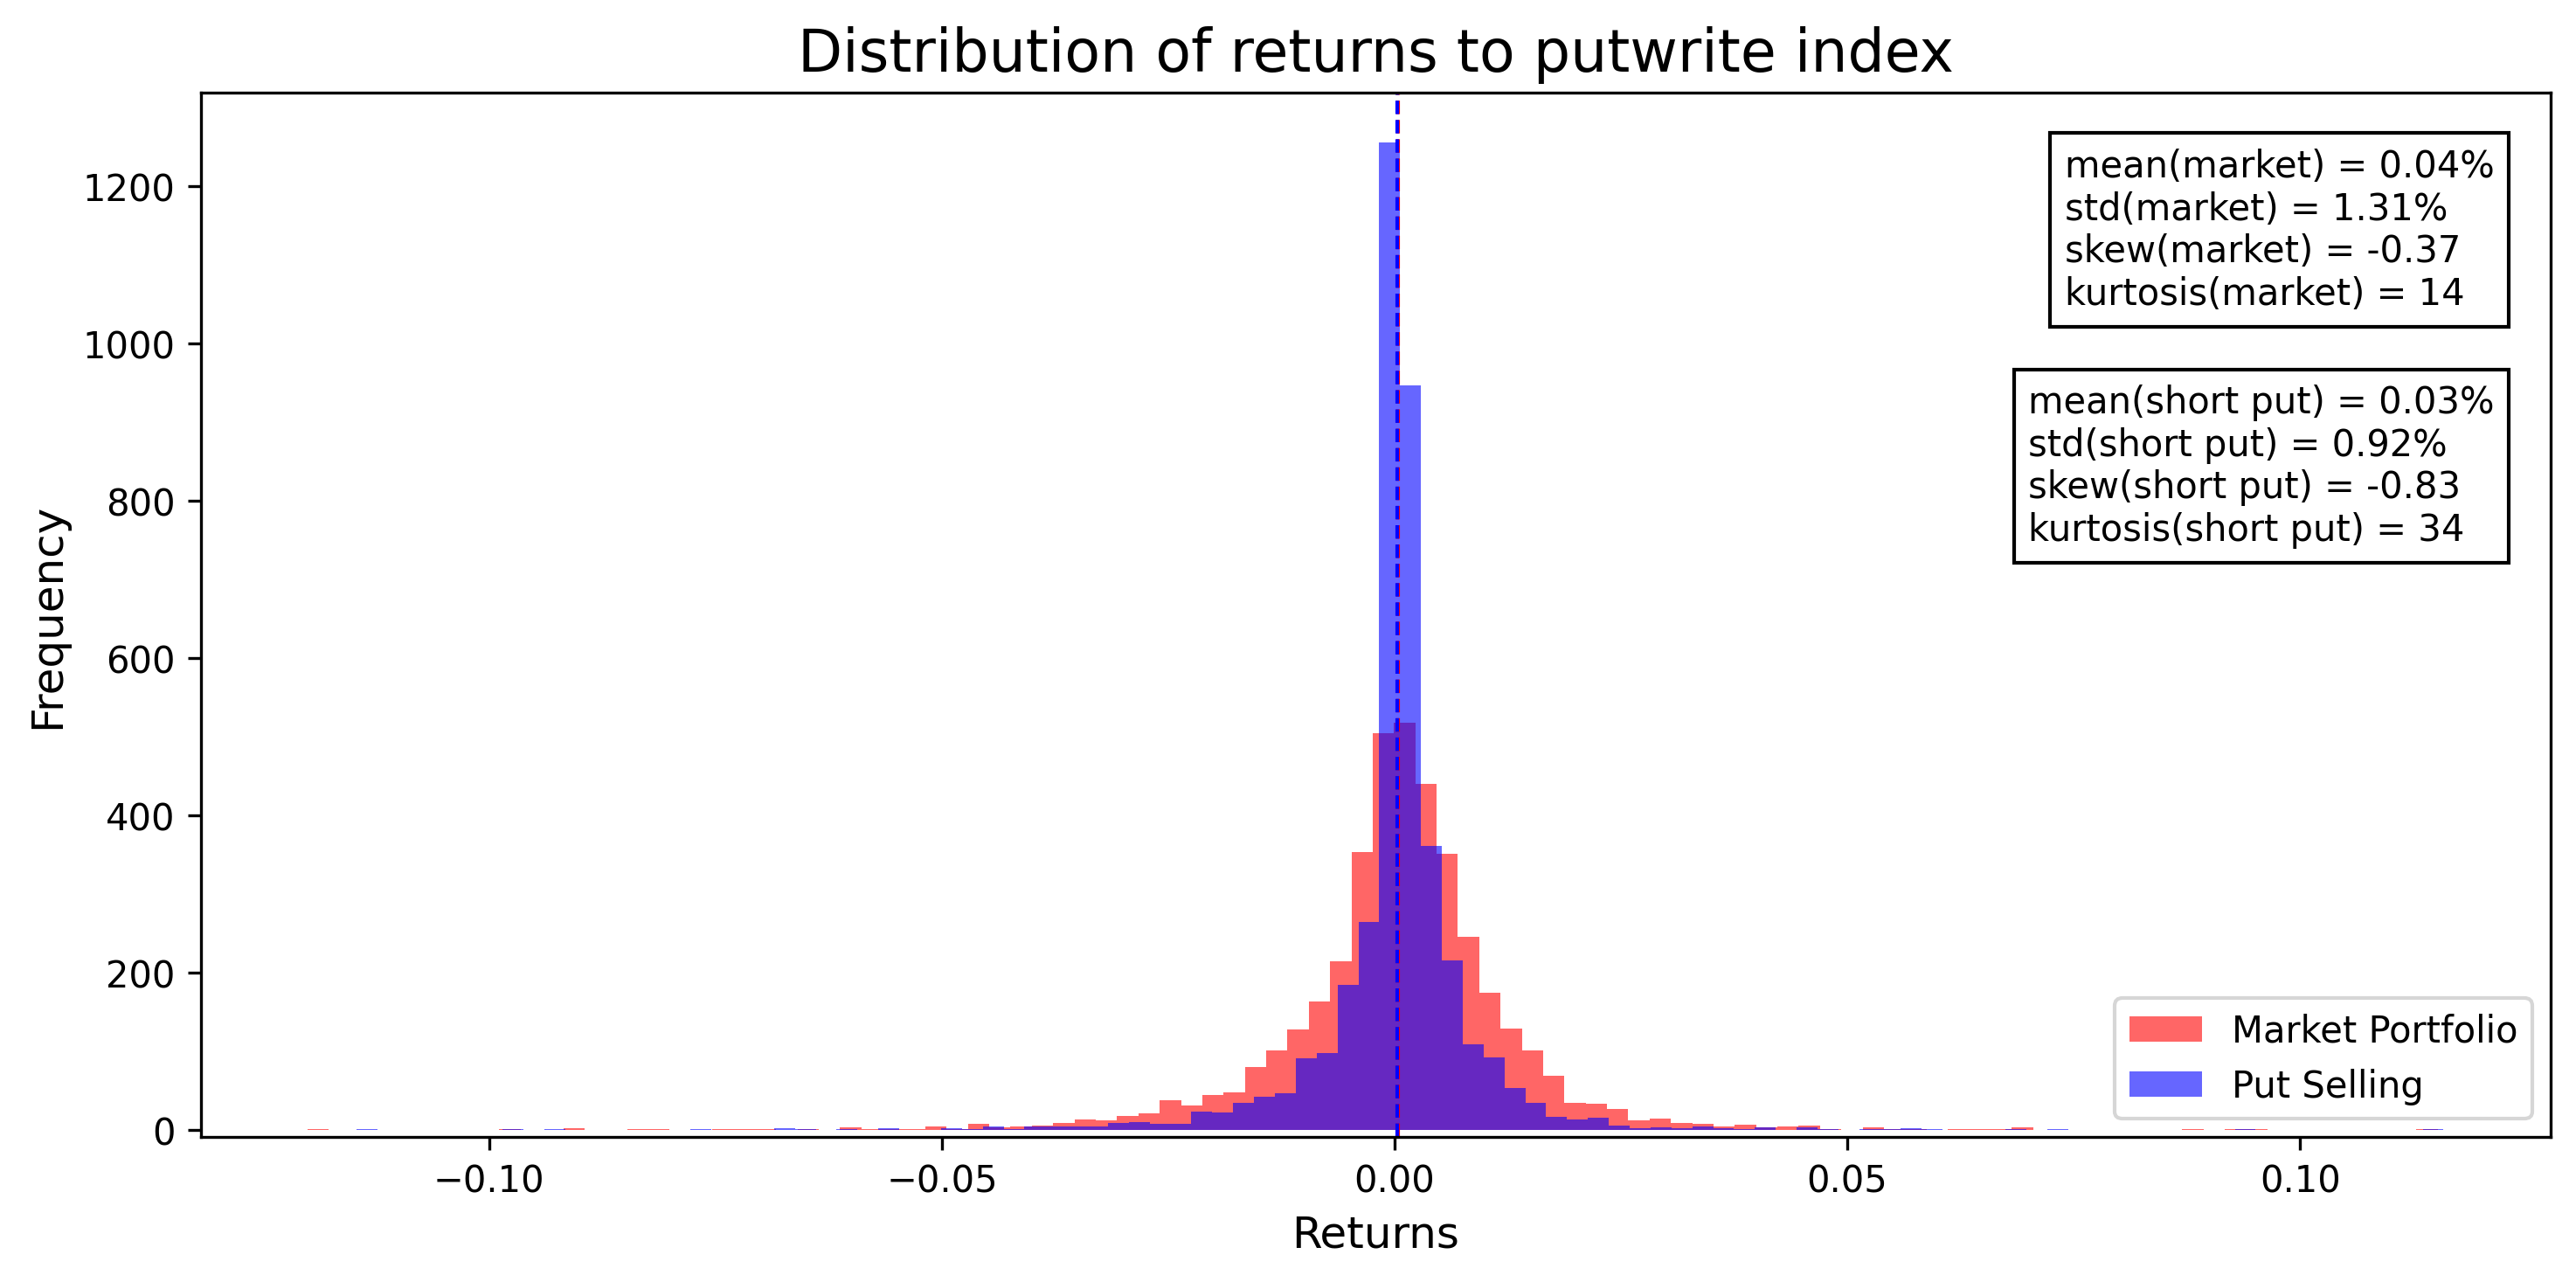
\includegraphics[width=0.75\textwidth]{fig13.png}
    \caption{Return distribution: S\&P 500 vs. PutWrite strategy}
    \label{fig:fig13}
\end{figure}

However, \autoref{fig:fig14} reveals the hidden danger. Examining the outliers (defined as daily returns with an absolute value above $3\%$), we find that the extreme losses are about the same in both cases. For very low stock returns, the put-write strategy behaves like leveraged stock exposure, yet unlike direct stock investment, investors are not conditioned to \say{expect the unexpected}.

\begin{figure}[h]
    \centering
    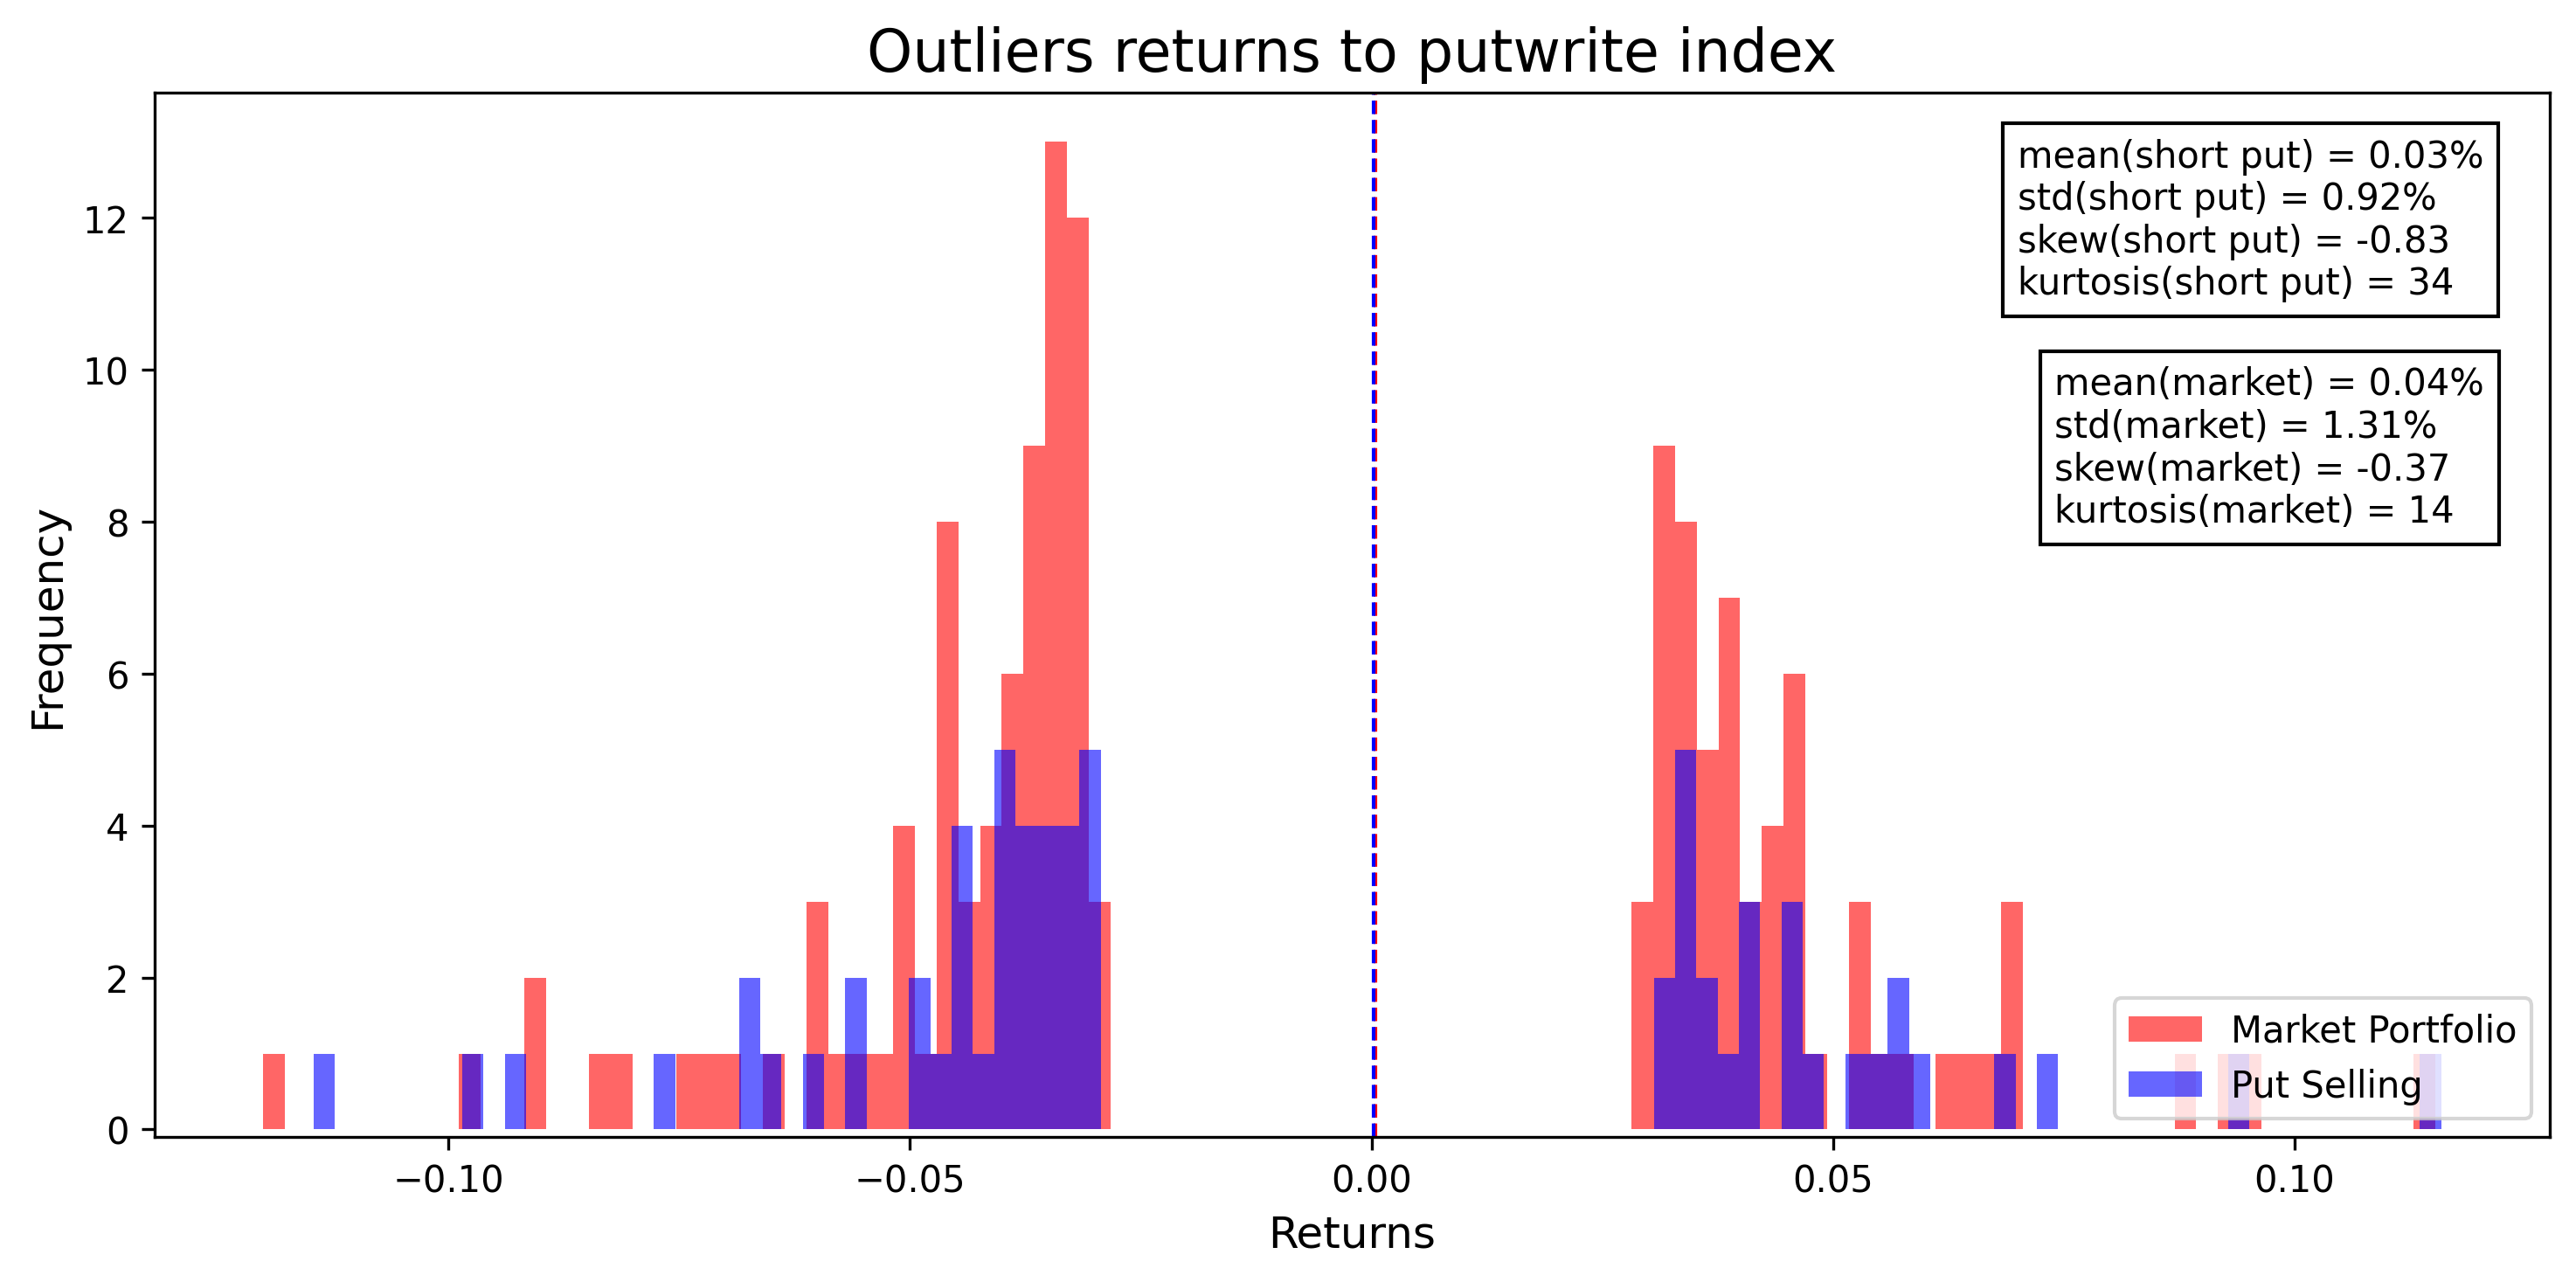
\includegraphics[width=0.75\textwidth]{fig14.png}
    \caption{Outlier returns}
    \label{fig:fig14}
\end{figure}

One might argue that sophisticated investors writing puts understand these risks and don't need such warnings. However, there is a deeper notion in which put options reveal the chicken narrative. First, the day-to-day payoffs represent the chicken before its neck is wrung, as steady small gains can mask hidden risk. The concentrated return distribution in Figure 13 shows this deceptive calm. Second, and more fundamentally, investors fell victim to the same type of model failure we saw in Section 5.2. Despite evidence of fat tails, many continued to rely on lognormal distribution assumptions that systematically underestimated tail risk.

The strategy's statistical properties (i.e., high frequency of small gains punctuated by rare large losses) are psychologically designed to encourage overconfidence in empirical patterns. Even sophisticated investors can fall prey to the same inductive reasoning that doomed Russell's chicken. They ignored the uncertainty outside their models and, as a result, were unprepared when that uncertainty manifested.


\subsection{The Chicken Problem is Everywhere}
The chicken problem extends beyond put options to other financial instruments with similar payoff structures.

Many accounts of the 2008-2009 crisis stress the role of credit default swaps. Market participants use credit default swaps to insure against default of a single entity, like a large financial institution, or baskets of corporate entities. Similar to life insurance, the protection buyer pays a periodic premium (called the spread) until maturity or default, and if the reference entity suffers a credit event, the writer compensates the buyer for the loss.

The CDX is an index of credit default swaps where market participants wrote contracts, known as tranches, that paid off depending on how many constituents of the CDX defaulted. The most super-senior of these tranches would only be affected if a large set of firms in the index defaulted simultaneously. 

\autoref{fig:fig15} \citep{seo2018rare} shows the time series of spreads on CDX super-senior tranches. Notice how spreads remained in the single digits from the onset of data availability through mid-2007, at which point they climbed as high as 80 basis points, increasing in 10-fold before 2008. This dramatic increase reflected a fundamental reassessment of systemic risk that market participants had previously underestimated. While some variation in spreads is expected, this pattern provides evidence that few market participants factored in the probability of an economy-wide crisis. Once again, steady returns on an asset that served as a substitute for cash lured investors into ignoring tail risk. Once again, an event outside of the model took market participants by surprise. 

\begin{figure}[h]
    \centering
    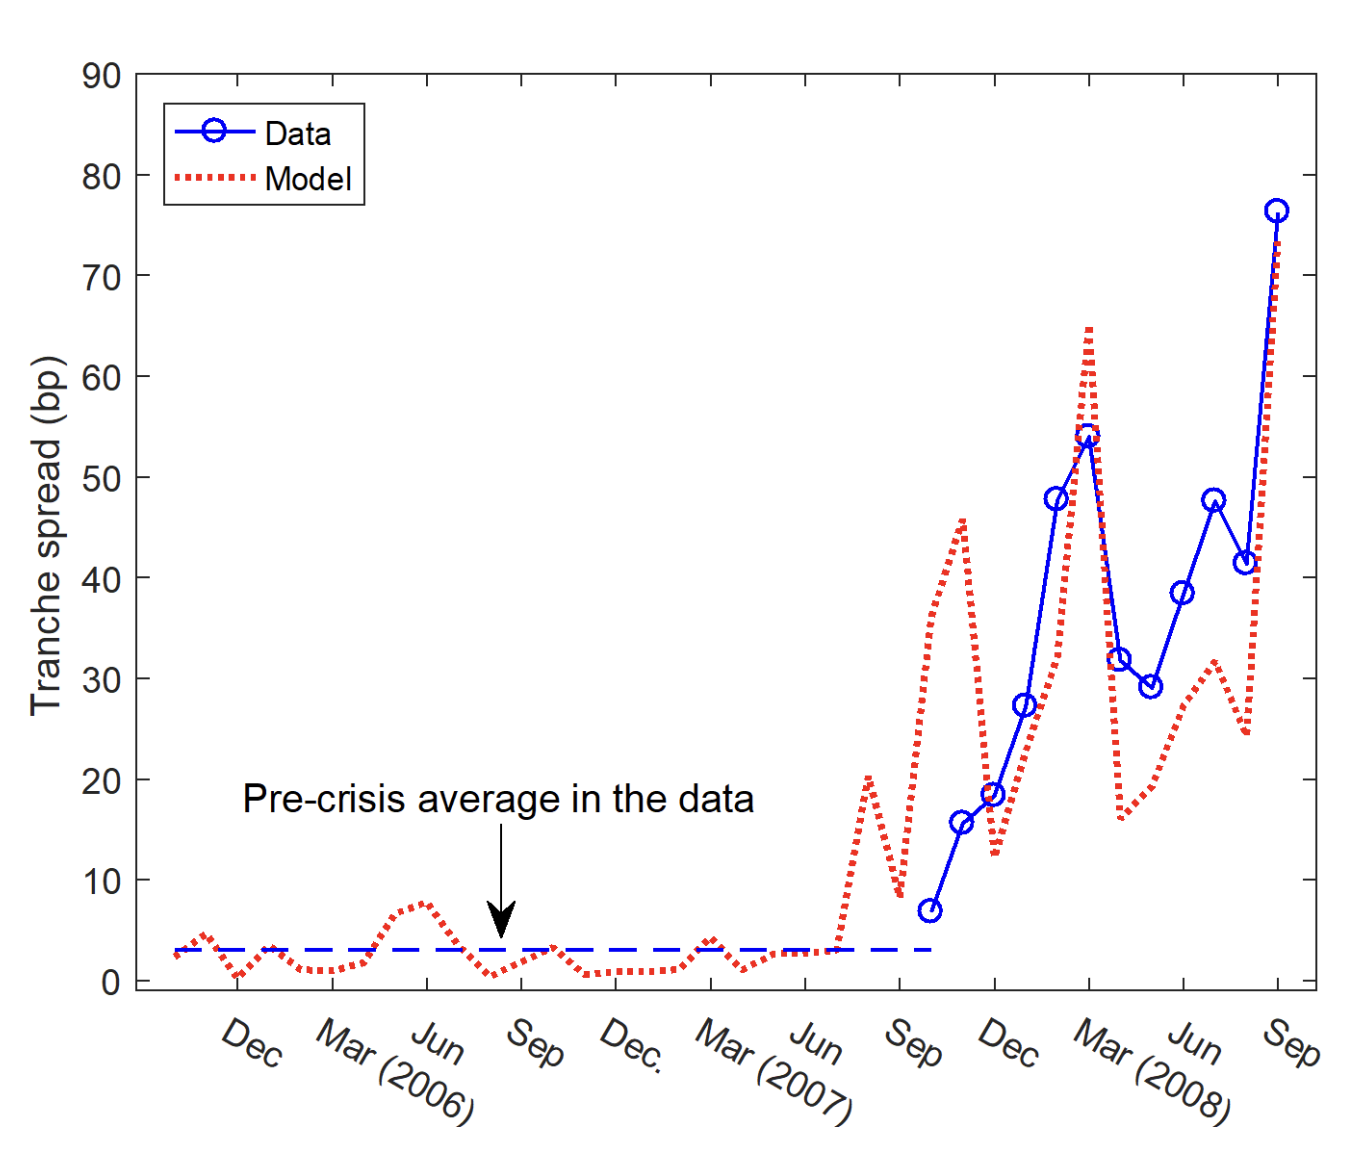
\includegraphics[width=0.75\textwidth]{fig15.png}
    \caption{Super-senior CDX spreads pre- and post-crisis \citep{seo2018rare}}
    \label{fig:fig15}
\end{figure}

Super-senior tranches exhibit the same deceptive pattern as Russell’s chicken: years of steady, small spreads followed by sudden catastrophic losses. Like put writers, investors collected modest premiums while remaining exposed to devastating tail events they systematically underpriced. 

The chicken problem extends even further through the fundamental structure of debt itself. Put-call parity shows that holding debt is mathematically equivalent to combining a risk-free bond with a short put position. Specifically, $\text{Debt} = \text{Riskless Bond} - \text{Put Option}$. Debt holders are essentially short put writers on the firm’s assets. If a firm’s value falls below the face value of its debt, debt holders suffer losses (exactly like put option writers when the underlying falls below the strike). Thus, put-like payoffs apply to all forms of lending: corporate bonds, bank deposits, short-term funding, and any other debt instrument. 

These embedded put options create interconnected vulnerabilities throughout the financial system. Short-term debt amplifies this problem through run dynamics. When concerns about solvency arise, creditors can withdraw funding quickly, forcing fire sales and creating the very losses that they feared.

This reveals why financial crises spread so quickly and broadly. The 1987 options market crash exposed a fundamental structure present throughout finance. Wherever there are promises to pay fixed amounts (debt), there are hidden put options. The chicken problem, with its deceptive pattern of steady gains masking tail risks, is not an anomaly but rather an inherent feature of modern financial systems.

The lesson from Russell's chicken applies far beyond any single strategy: when steady feeding suddenly stops, the consequences can be catastrophic and system-wide.

\section{Discussion}
The pattern documented in our analysis, from the 1987 crash to the persistent chicken problem across various debt securities, raises a fundamental question: why do market participants repeatedly fall into these traps?

The model that we started with suggests that individuals make probability calculations when they make decisions. Researchers have long pointed out, however, that individuals fail at even the most straightforward probabilistic calculations. Even colloquially, “the expected” often means “what comes to mind” rather than an actual calculation. This is not to suggest that people do not use models, such as the Black-Scholes-Merton model, or the copula models widely in use for the CDX contracts. Rather, they neither take these models seriously as true pictures of the world, not subjecting them to scrutiny that that would entail, nor do they form any conscious model, but rather make decisions based on what comes to mind. 

In the study of economics, we often seek to measure and to model this uncertainty, and the first step is typically a simplification. When we create a random variable, we are replacing a multi-, potentially infinite-dimensional object with something that has a fixed number of dimensions. Moreover, the idea of “expectation” (calculated as $E[X]$) has a strange consequence that the expected never happens: if you paid \$1 to earn \$2 if a coin were heads and \$0 if tails, you expect to earn \$1 on net from this gamble, yet that outcome can never occur. 

Perhaps we need a different way of thinking about finance and the unexpected. Recent research turns to evidence on memory to understand expectations. Our memories, and thus our thoughts and beliefs, are driven by: recency, similarity, and temporal contiguity.

Economists have long noted the strong pull of recent events on expectations. Recall that one of the questions that we are uncertain about was the return on the stock market (from Section 1). Several long-running surveys capture beliefs about this question. The Gallup survey asks respondents if they are very optimistic, optimistic, neutral, pessimistic, or very pessimistic. Campbell Harvey and co-authors surveyed CFOs about their expectations of stock returns over the next 12 months. These and more surveys were reviewed in a paper by \citet{greenwood2014expectations}.


\autoref{fig:fig16} \citep{greenwood2014expectations} shows the percentage of investors who are very optimistic or optimistic minus the percentage of investors who are pessimistic or very pessimistic, compared to stock returns from 12 months prior. The difference in this measure is well explained ($r^2 = 61 \%$ for Gallup) by returns from 12 months prior. Needless to say, this is not a good model for stock market returns. If anything, stock returns in aggregate exhibit negative autocorrelation over the relevant horizons. Recent events strongly influence the survey responses of these individuals. 

\begin{figure}[h]
    \centering
    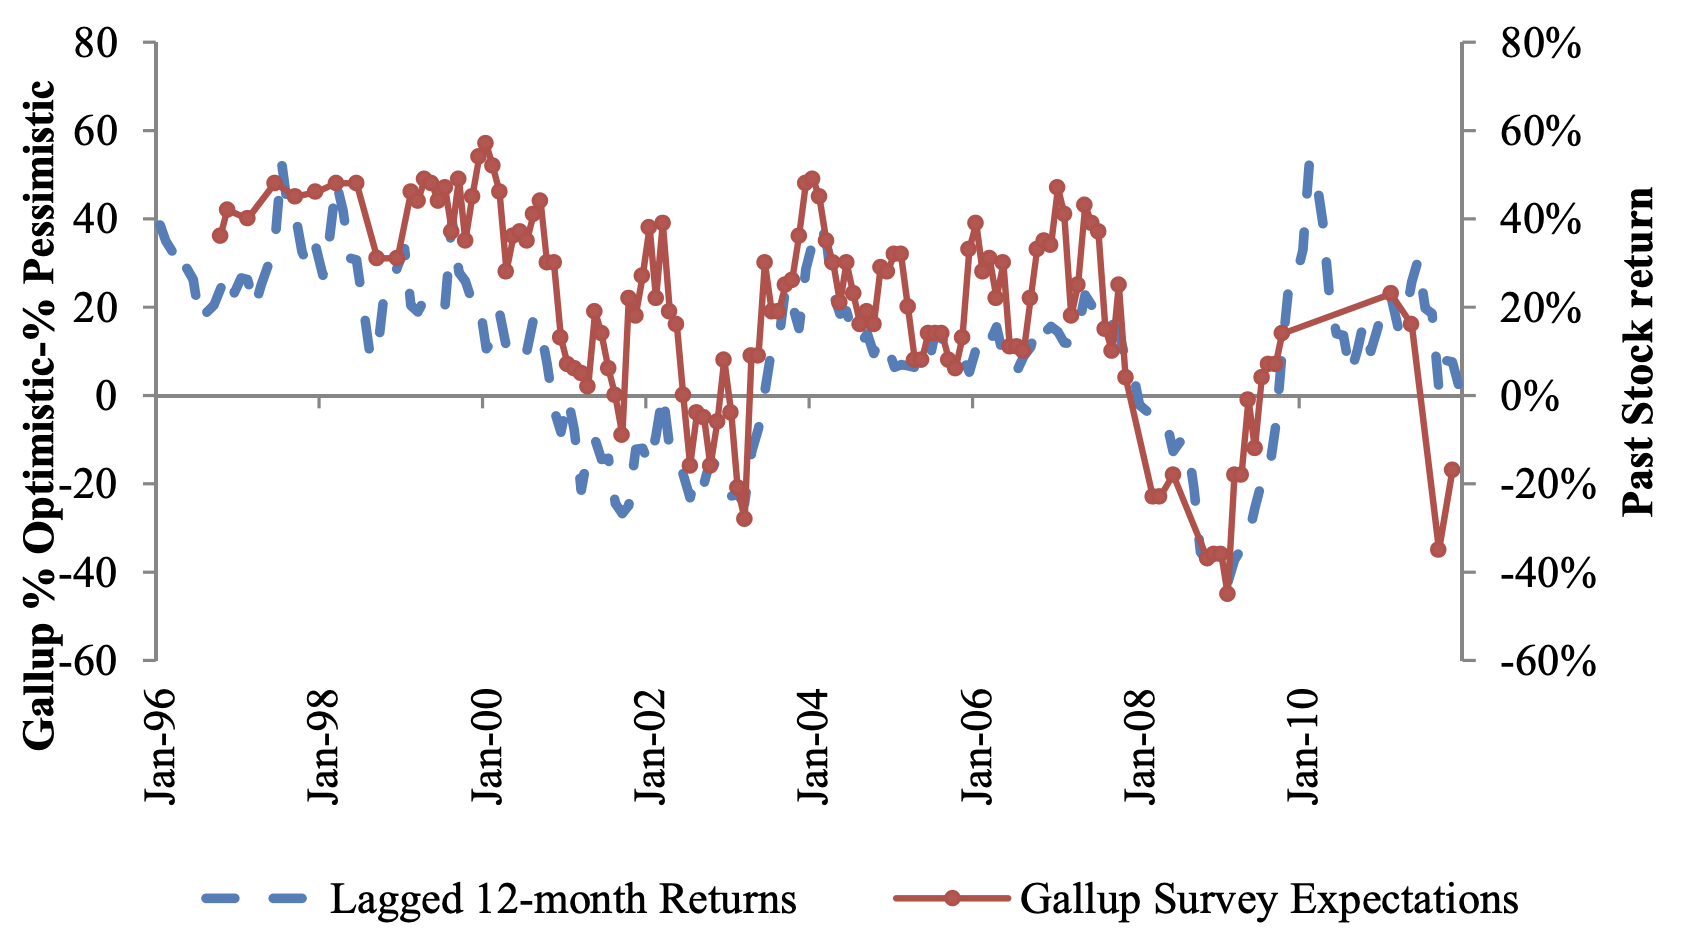
\includegraphics[width=0.75\textwidth]{fig16.png}
    \caption{Gallup survey responses compared to shifted stock returns \citep{greenwood2014expectations}}
    \label{fig:fig16}
\end{figure}

Recall the problem faced by the chicken. Even with no recency bias, it is difficult to infer the underlying distribution of events when faced only with data and with an incorrect model. A little imagination might have helped the chicken. However, if our beliefs are pulled toward recent events, that will make it even more difficult to have this imagination.

There are some important caveats to recency, as recent experiences are a subset of experience. Researchers have also shown that experience matters, both past and present. One 2009 study showed that experience moderates the effects of recency \citep{greenwood2014expectations}. The authors studied asset managers' holdings during the dot-com bubble by regressing change in holdings in technology stocks on age in each quarter. \autoref{fig:fig17} \citep{greenwood2009inexperienced} shows the coefficients plotted against the returns in that quarter. They found that the dependence on past returns decreased, the older the asset manager. That is, younger managers tended to chase trends whereas older ones were contrarians. The higher the returns, the more likely it is younger managers investing and older managers dis-investing.

\begin{figure}[h]
    \centering
    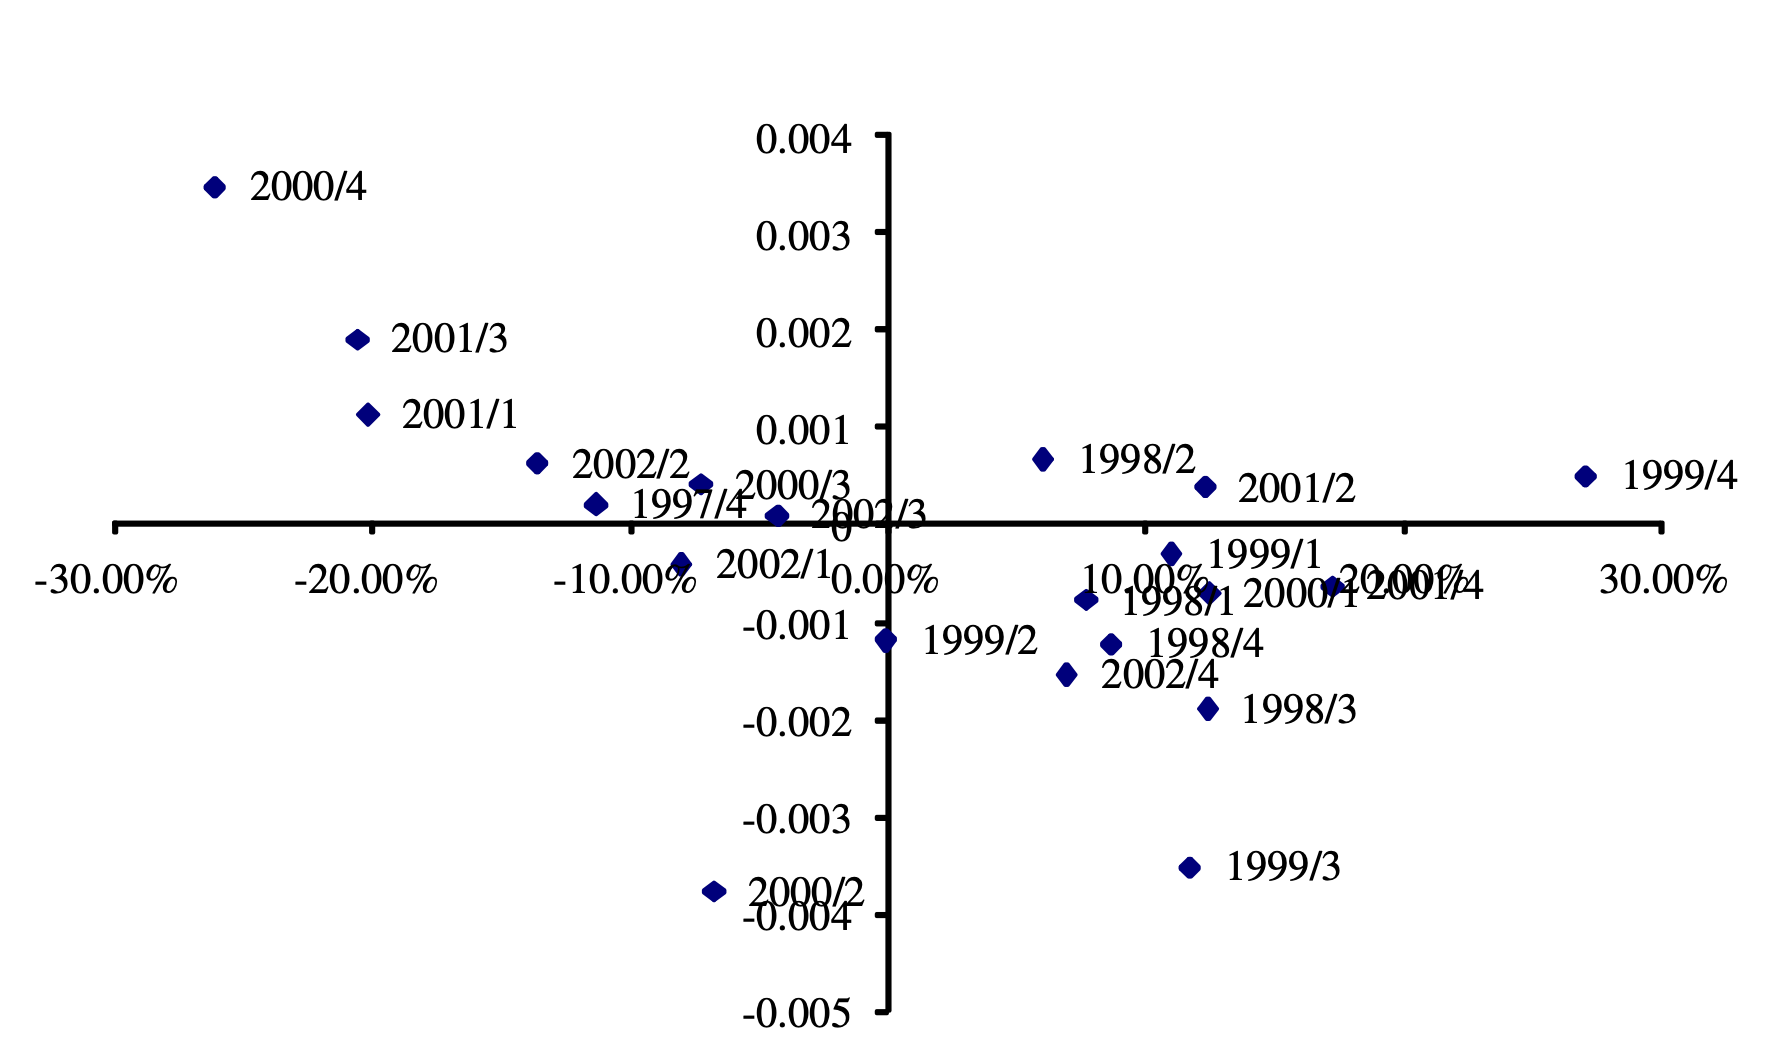
\includegraphics[width=0.65\textwidth]{fig17.png}
    \caption{Regressing age with change in managers' holdings \citep{greenwood2009inexperienced}}
    \label{fig:fig17}
\end{figure}

This study has the remarkable conclusion that early life experience in the stock market is apparently never forgotten. The importance of experience is a link between financial decisions, and the relevance of free recall in the laboratory. Because if experience matters, then memory matters. And free recall is the study of memory.

When an event is recalled, memory is biased toward other events that occurred close in time. This clustering effect is called temporal contiguity \citep{howard2002distributed}. Temporal contiguity is thought to arise because recalling an item reinstates the mental context from when it was first learned, and that reinstated context makes nearby memories easier to access.

According to context-maintenance models of memory, individuals’ thoughts and beliefs are governed by an internal context. Information from the environment retrieves a context that depends on the features filtered through past memories: the individual retrieves past contexts in which similar features were experienced. Retrieved context averages with past context to form current context. Current context determines what comes to mind. This framework helps explain why we sometimes struggle to recall specific details while also accounting for the fact that memories are rarely lost entirely.

Moreover, mental context has broader implications for decision-making. Associations formed in one context can lead to very different responses than those formed in another. As underlying mental associations evolve, the decisions that stem from them can change as well. Deciding how to invest and how much are some of the most important financial decisions an investor can make. Recent literature has turned to the role of lifetime experience in shaping these choices. \citet{malmendier2021memory} show that lifetime stock market performance is a major determinant of whether an individual chooses to participate at all (\autoref{fig:fig18}). People with better lifetime market experiences (e.g., those in the 90th percentile of lifetime market performance) are 10 percentage-points more likely to invest than those with worse experiences (e.g., those in 10th percentile), in a sample where the average participation rate is 34\%. The magnitude of these experience effects is comparable to that of other well‑established determinants, including income and education.

\begin{figure}[h]
    \centering
    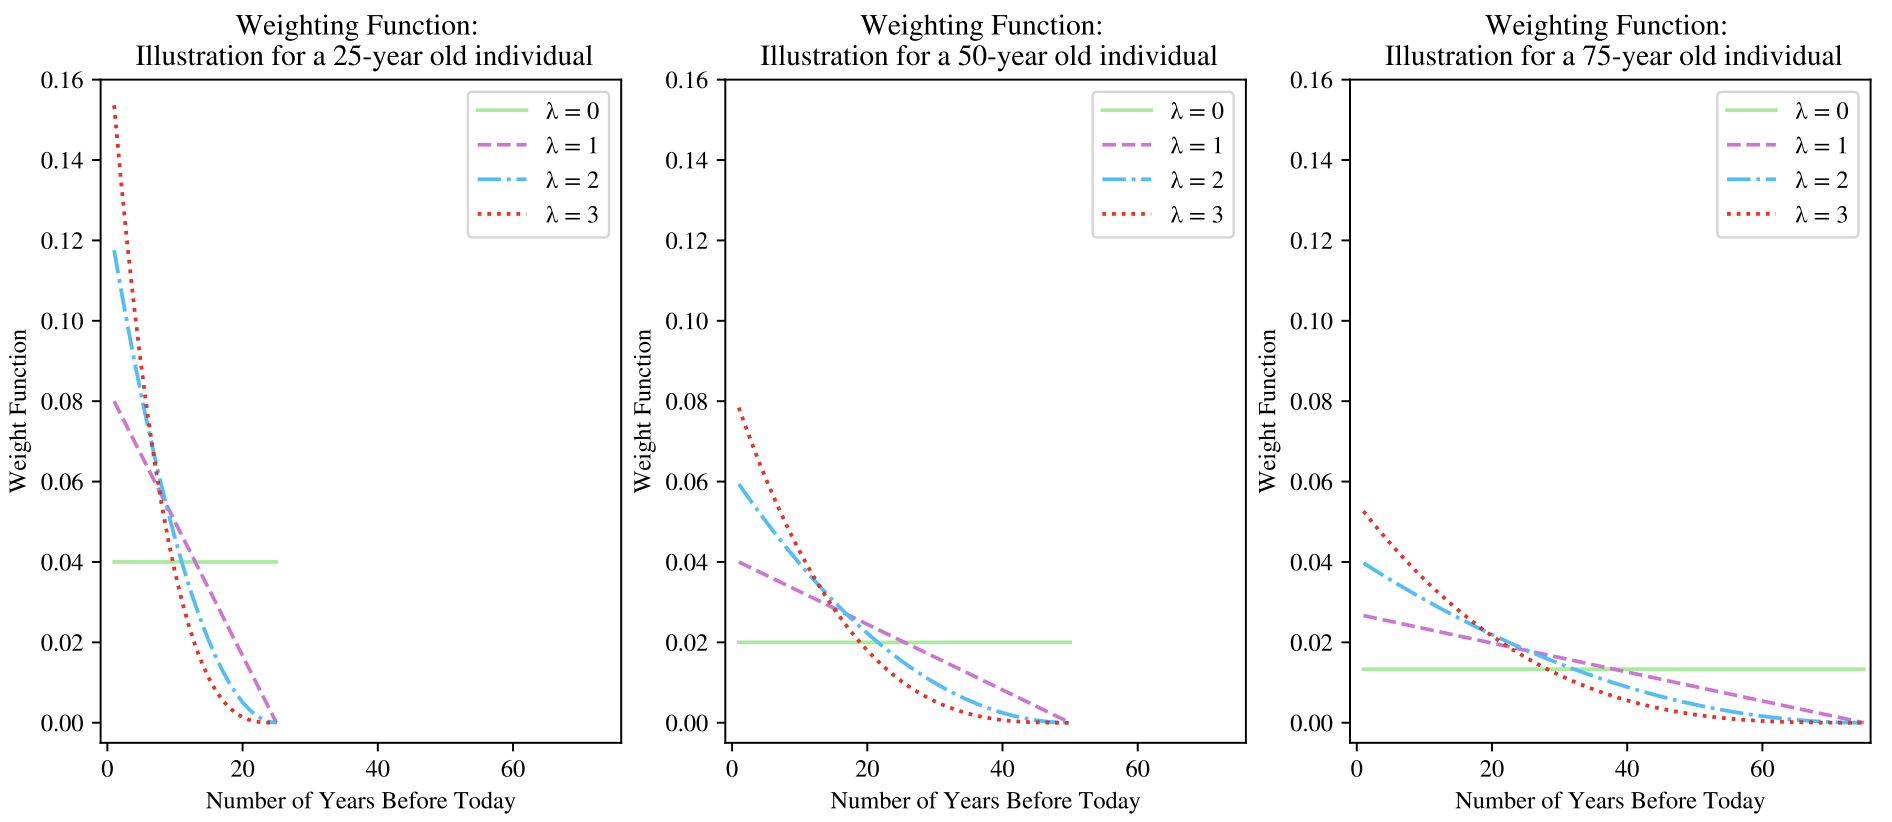
\includegraphics[width=0.75\textwidth]{fig18.png}
    \caption{Weight of past experiences changes with age \citep{malmendier2021memory}}
    \label{fig:fig18}
\end{figure}

Multiple findings relevant to financial data reflect these results. \citet{guiso2018time} examined risk aversion in an experiment with the same set of participants before and after the 2008 crisis. The participants, who were professional traders, required twice the premium to accept a bet following the crisis as before. The people were the same, the bets were the same, but the associations had changed. The same study also performed an experiment in which undergraduates watched a scene from a horror movie: those who watched the scene required a 50\% greater premium to invest than those that did not. 

Another study \citep{cohn2015evidence} experimentally manipulated context by presenting study participants, who were professional traders, with scenarios involving a normal trading day versus a stock market crash. The traders were then presented with risky bets with various degrees of return. Those with the market crash context required a higher premium to accept the risky bet. Both the horror movie and crash simulations represented context manipulations that affected behavior.  
 
Ultimately understanding the unexpected in finance means grappling with the unexpected in human decision-making. We believe that research in memory offers one path forward.

\section{Conclusion}
To bring this back to where we started, we saw that individual stock returns exhibit positive skewness that can be phased by diversifying. This requires markets, and specifically public equity issuance, which requires the amelioration of moral hazard\textemdash something regulation can accomplish. The aggregate market is still risky (exhibits excess kurtosis), yet we do know that it is not well-described by a normal distribution. Besides heavy tails, aggregate market returns exhibit negative skewness, implying that negative events tend to go together.

Option prices reflect these heavy-tailed returns, though they did not always, reflecting another source of uncertainty: uncertainty in models. Models are important because judging the future purely by past events without understanding leaves us exposed to the chicken problem. We can be lured by a safe time series into thinking that nothing bad will happen; we can also be lured into believing a model representing safety is correct if we are not willing to consider alternatives. If our beliefs are confounded by recency bias, this will be difficult, and research shows that recent events, especially if they are noticeable like stock returns, do inform beliefs and survey responses. But a closer look shows that the entire lifetime of experience matters, paving the way for a memory-based model.

Yet the most remarkable finding may be what was truly unexpected: the extraordinary performance of the stock market over the last 100 years. While daily returns on the aggregate market are negatively skewed, the distribution of long-run returns is highly positively skewed. One dollar invested grows more than four-fold, even adjusting for inflation as shown in \autoref{fig:fig19} \citep{binsbergen2023united}. This is a remarkable success story that would have come entirely as a surprise back in the $1920s$. The idea that one might give a risky venture money and expect to be paid off is surprising, but it is regulation that controls, for example, the moral hazard problem, that makes this possible.

\begin{figure}[h]
    \centering
    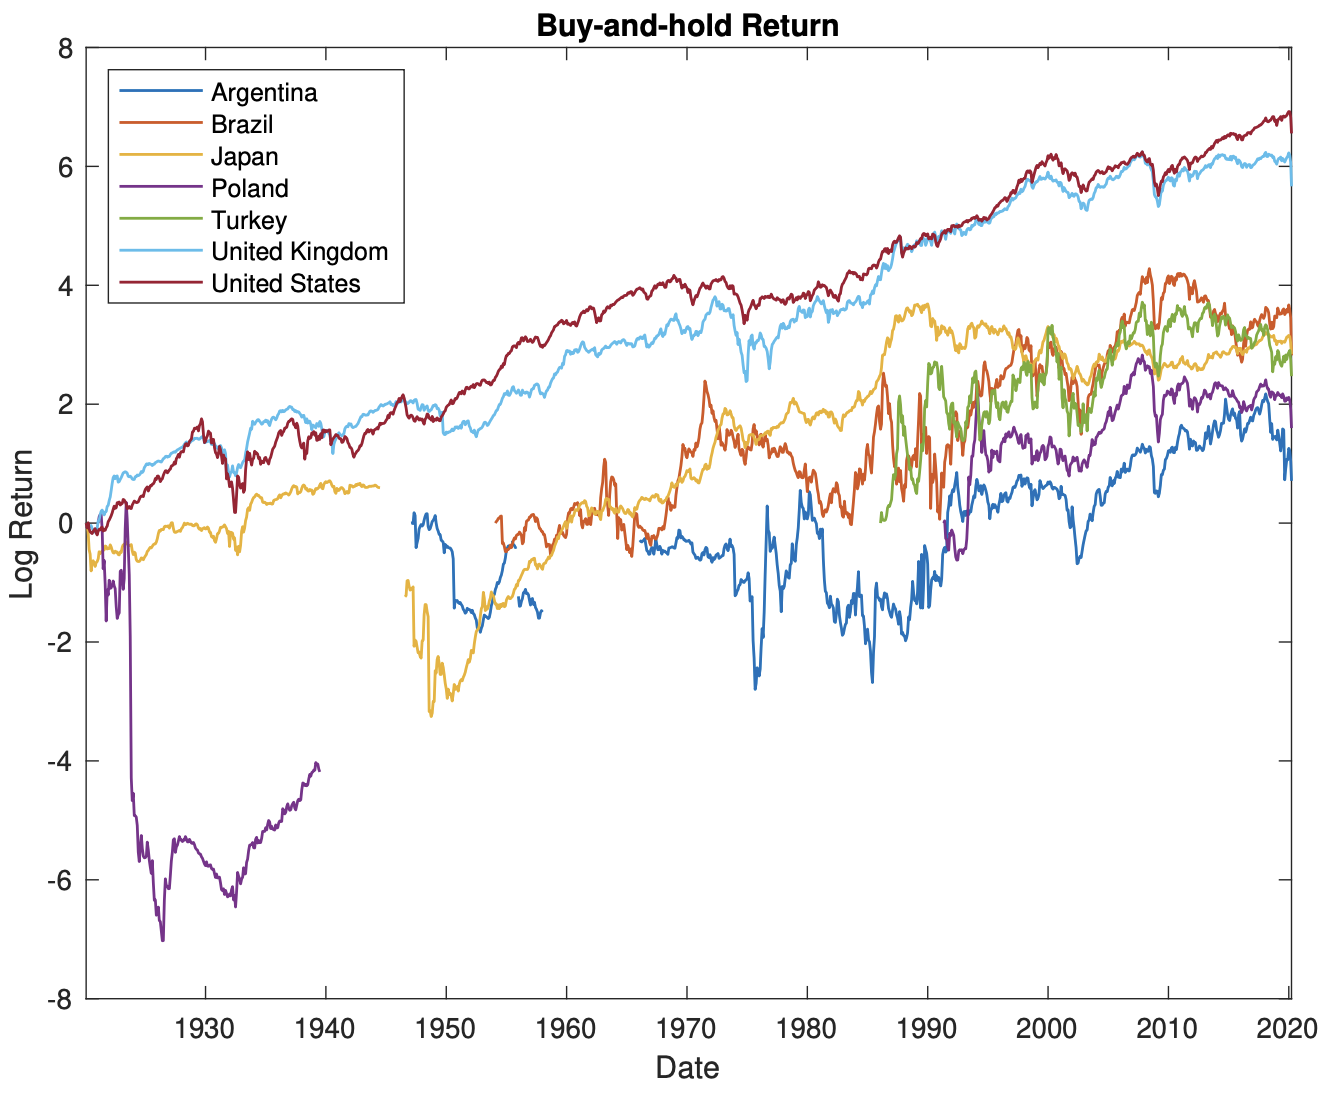
\includegraphics[width=0.75\textwidth]{fig19.png}
    \caption{Stock market returns \citep{binsbergen2023united}}
    \label{fig:fig19}
\end{figure}

Decades of research have failed to account for this based on standard methods of risk. Rather, it appears that this was a continuous surprise. It is a remarkable story, and an unexpected one, that reforms set up in the $1930s$ and $1940s$ would have worked so well in allowing capital to grow. In the long run, skewness in market returns is positive, not negative. The unexpected was this positive event, that a regulatory regime established in the $1930s$ and $1940s$ would work so surprisingly well. Understanding this tension between short-run tail risks and long-run positive surprises may be the most important lesson finance has to offer. 




\appendix
\section{Code and Data Availability} \label{appendix:code}

All the code and data used in this study are available at the following GitHub repository: \\
\url{https://github.com/anantapantulasa/unexpected_finance}


\bibliographystyle{plainnat} % can replace with apa or mla! 
\bibliography{references}

\end{document}